\chapter[\hspace{0pt}基于语义-视觉多空间关系建模的少样本分类研究]{{\heiti\zihao{3}\hspace{0pt}基于语义-视觉多空间关系建模的少样本分类研究}}\label{chapter4: 基于语义-视觉多空间关系建模的少样本分类研究}
\removelofgap
\removelotgap

上一章研究了基于多粒度样本关系建模的少样本特征学习算法,通过充分挖掘不同粒度的样本关系提高了网络所提取特征的质量。然而,该算法仅在视觉空间对多种样本关系进行了建模,忽略了数据集中所隐含的丰富语义信息,限制了模型通过基类数据进行训练来学习新类数据知识的能力。因此,在上一章的基础上,本章主要研究基于语义-视觉多空间关系建模的少样本特征适配算法,通过引入语义信息并与视觉信息进行建模从而丰富模型所获得的信息,增强模型的泛化能力。本章内容共分为四节,\hyperref[section4: 引言]{第一节}介绍研究动机和方法概述;\hyperref[section4: 基于语义-视觉多空间关系建模的少样本特征适配算法]{第二节}介绍本章提出的基于语义-视觉多空间关系建模的少样本特征适配算法;\hyperref[section4: 实验设置及结果分析]{第三节}给出实验设置和结果分析;\hyperref[section4: 本章小结]{第四节}对本章进行小结。

\section[\hspace{-2pt}引言]{{\heiti\zihao{-3} \hspace{-8pt}引言}}\label{section4: 引言}

\subsection[\hspace{-2pt}研究动机]{{\heiti\zihao{4} \hspace{-8pt}研究动机}}\label{section4: 研究动机}

基于视觉的少样本算法,包括基于元学习、度量、数据增强、以及特征学习的方法已经取得了显著进展。然而,这些方法仍面临一些局限性,影响了模型性能的提升。特别是,这些方法往往仅关注样本的视觉信息,忽视了语义信息的潜在价值,使得模型难以从少量样本中学习到具有足够泛化能力的特征表示,这一点直接制约了模型对新类别的识别能力,限制了模型的性能上限。

\begin{figure}[h!]
  \centering
  \captionsetup{font={small, stretch=1.312}}
  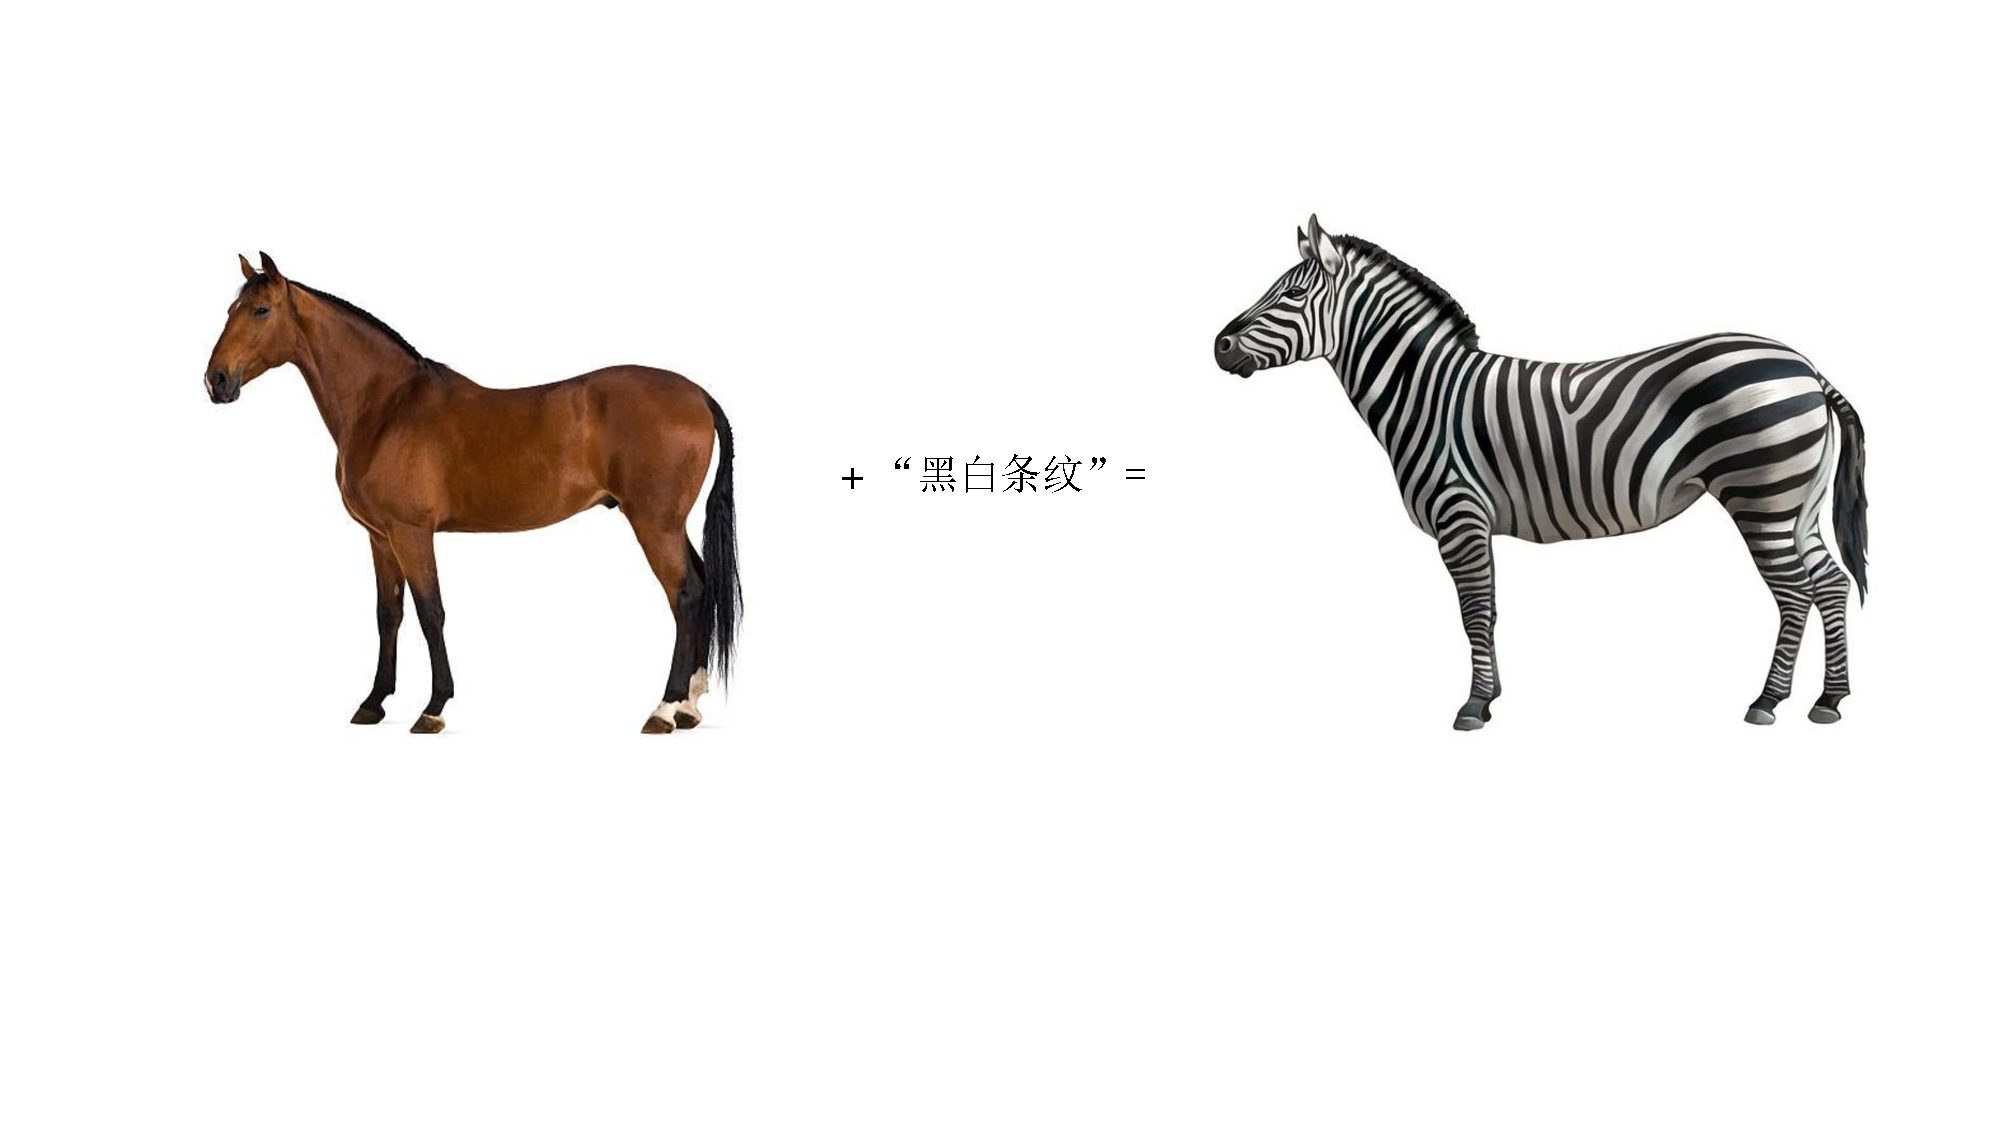
\includegraphics[width=0.9\columnwidth]{figures/SVMSMA/人类认识新类别示意图.pdf}
  \bicaption[人类认识新类别的过程示意]{人类认识新类别的过程示意。以斑马为例进行说明。}[Human process for recognizing new categories]{Human process for recognizing new categories. Illustrated by the example of a zebra.}
  \label{figure4: 人类认识新类别示意图}
\end{figure}

与深度学习模型不同,人类在认识新类别时,依赖的不仅是视觉形象,更多的是对于该形象背后语义的理解和推理。例如,告知某人“斑马”是一种有黑白条纹的“马”,即使在没有看到斑马的情况下,该人也能凭借对“马”的认知和对“黑白条纹”的描述,快速理解并识别“斑马”,如图\ref{figure4: 人类认识新类别示意图}所示。这种通过语义信息桥接的学习过程,是人类认识新事物的一大优势,也是机器学习中尚待深入挖掘的宝贵资源。受到人类认识新物体的启发,研究者认为语义信息在计算机视觉任务中也可发挥同样的作用,尤其是在零样本分类\cite{metric1, metric2, generative1, generative2, 冯耀功2020基于知识的零样本视觉识别综述, 零样本学习, 赵鹏2021一种基于融合重构的子空间学习的零样本图像分类方法}以及少样本分类\cite{KTN, AM3, TRAML, yan2021aligning, CMGNN-DPGN, STVAE, SP-CLIP, 赵凯琳2020小样本学习研究综述, 刘颖2021基于小样本学习的图像分类技术综述, 小样本困境下的深度学习图像识别综述}任务中。为了模拟人类认识新类别的过程从而更好地建立新类与基类之间的联系,很多研究者开始使用自然语言模型\cite{Word2Vec, GloVe, Bert}或多模态模型\cite{Clip}的文本编码器提取类别名称的语义特征作为语义信息,并将其用到少样本分类方法中,如\ref{section1: 研究现状}中所述。


然而,这些工作虽在少样本分类任务中引入了语义信息并进行有效利用,但仍存在一些不足。部分基于特征生成的方法,如STVAE\cite{STVAE}使用语义信息作为条件训练一个特征生成模型。在训练好特征生成模型后,为了提高少样本测试任务中的样本多样性,需要向支持集中添加大量样本,这一做法使得后续的分类器训练时间急剧增长。并且部分生成模型训练过程较为复杂,例如生成对抗网络(Generative Adversarial Networks,简称GAN)\cite{GAN}在训练时需要交替训练生成器和判别器;以及扩散模型(Diffusion Model)\cite{diffusion}在训练时则是需要逐步加噪和去噪过程。基于语义修正的方法\cite{AM3, SP-CLIP}虽然不需要在进行少样本测试任务时对支持集样本进行扩充,但这些方法往往需要设计精细且复杂的信息融合模块,并且这些模块的设计还可能会对自然语言模型或多模态模型所提取的语义信息产生不利影响。具体来说,自然语言模型或多模态模型在大规模语料库上进行了训练,因此提取的语义特征具有较强的泛化性,而过于复杂的信息融合模块可能使得模型在基类数据集产生过拟合问题,削弱这种泛化性,进而降低模型的整体表现。


\subsection[\hspace{-2pt}方法概述]{{\heiti\zihao{4} \hspace{-8pt}方法概述}}\label{section4: 方法概述}

为解决上述问题并充分利用语义信息以补充视觉信息,进而提升少样本分类任务的准确率,本章提出了一种基于语义-视觉多空间关系建模的少样本特征适配算法,即语义-视觉多空间映射适配(Semantic-Visual Multi-Space Mapping Adapter,简称SVMSMA)模型。SVMSMA模型以一种简单的特征适配方式利用语义信息,不需要对语义特征进行复杂信息融合操作,从而避免了降低语义特征泛化性的问题,并能够有效丰富样本特征的信息来源,弥补仅使用视觉信息的不足。

由于在少样本分类测试任务中,查询集只能够获得视觉信息(已知语义信息则已知类别),为了执行测试任务以及使用跨模态分类任务(将在后续介绍)对网络进行优化,本文采用将语义信息映射到视觉空间的方案对两种信息之间的关系进行建模。因此,本文首先提出了一个语义-视觉多空间映射网络(Semantic-Visual Multi-Space Mapping Network,简称SVMSMN),采用两种可独立使用的模式将语义信息映射到视觉空间:1)单模态映射,2)多模态映射。单模态映射是指使用类似零样本学习的思想,仅将语义信息映射到视觉空间,在执行测试任务时仅使用语义信息来获取语义映射特征,并不会使用到支持集样本的视觉特征。多模态映射则是在语义信息的基础上使用视觉信息对其进行补充,将两个模态信息融合后再映射到视觉空间,以对支持集样本的视觉信息加以利用。

另外,为了建模语义信息与视觉信息的关系,从而能够使用语义映射特征对支持集的视觉特征进行补充,提升少样本分类任务性能,本文提出了两个模块以对语义-视觉多空间映射网络进行优化使得语义映射特征适配视觉空间,分别是1)跨模态分类(Cross-Modal Classification,简称CMC)模块,2)跨模态特征对齐(Cross-Modal Feature Alignment,简称CMFA)模块。其中,跨模态分类模块使用预训练的视觉特征提取网络的分类器对上述语义映射特征进行分类,以对映射网络进行优化使得每个类别的语义信息和对应的视觉特征建立联系。跨模态特征对齐模块则是将语义映射特征与通过视觉特征提取网络得到的视觉特征原型进行对齐,以这种方式对映射后的特征进行修正,使其更接近类别原型,从而能够取得更好的分类结果。

本章方法同样在四个少样本分类数据集进行了实验,包括miniImageNet\cite{vinyals2016matching}、tieredImageNet\cite{ren2018meta}、CIFAR-FS\cite{bertinetto2019meta},以及CUB-200-2011\cite{wah2011caltech}。实验结果表明,本章方法可有效建模语义-视觉空间关系,利用语义信息对视觉信息进行补充,从而取得优异的少样本分类结果。

\section[\hspace{-2pt}基于语义-视觉多空间关系建模的少样本特征适配算法]{{\heiti\zihao{-3} \hspace{-8pt}基于语义-视觉多空间关系建模的少样本特征适配算法}}\label{section4: 基于语义-视觉多空间关系建模的少样本特征适配算法}

在本节中,首先对使用语义信息的少样本分类任务及其符号定义进行介绍;然后对所提出的基于语义-视觉多空间关系建模的特征适配模型进行简要介绍;接下来详细介绍了所提模型的各个模块及其损失优化;最后介绍了模型总体优化目标以及模型推理过程。

\subsection[\hspace{-2pt}符号定义]{{\heiti\zihao{4} \hspace{-8pt}符号定义}}\label{section4: 符号定义}

在本章中,由于引入了语义信息,各种符号定义与第三章有所不同。基类数据集与新类数据集分别表示为:
\begin{equation}
  \begin{aligned}
     & \mathcal{D}_{base} = \{(x, y, s)|x \in X^{base}, y \in Y^{base}, s \in S^{base}\},     \\
     & \mathcal{D}_{novel} = \{(x, y, s)|x \in X^{novel}, y \in Y^{novel}, s \in S^{novel}\}.
  \end{aligned}
\end{equation}
其中,$\mathcal{D}_{base}$所包含的类别$\mathcal{C}_{base}$和$\mathcal{D}_{novel}$所包含的类别$\mathcal{C}_{novel}$不相交。另外,$x$、$y$、$s$分别表示样本图像、样本标签、以及样本语义特征;$X^{base}$、$Y^{base}$、$S^{base}$分别表示基类样本图像集合、标签集合、语义特征集合;$X^{novel}$、$Y^{novel}$、$S^{novel}$则分别表示新类样本图像集合、标签集合、语义特征集合。在本章中,语义特征是通过将类别名称/提示文本+类别名称输入自然语言处理模型或者多模态模型的文本编码器得到的。

与上一章相同,本章也通过在$\mathcal{D}_{novel}$中采样大量少样本分类任务并计算平均准确率来评估模型性能。不同的是,本章所采样少样本分类任务的支持集$\mathcal{S}_{\mathcal{T}}$除了包含样本图像$x_i$以及样本标签$y_i$外,还包含了样本语义特征$s_i$。因此,支持集表示为:
\begin{equation}
  \mathcal{S}_{\mathcal{T}} = \{(x_i, y_i, s_i)|x_i \in X^{\mathcal{T}}, y_i \in Y^{\mathcal{T}}, s_i \in S^{\mathcal{T}}\}_{i=1}^{N \times K},
\end{equation}
其中,$X^{\mathcal{T}}$、$Y^{\mathcal{T}}$、$S^{\mathcal{T}}$分别表示所采样任务的样本图像集合、标签集合、语义特征集合;$N$和$K$则是表示类别数目以及每个类别样本数目。查询集的样本类别未知,因此无法获取其语义特征,表示为:
\begin{equation}
  \mathcal{Q}_{\mathcal{T}} = \{(x_i, y_i)|x_i \in X^{\mathcal{T}}, y_i \in Y^{\mathcal{T}}\}_{i=1}^{N \times Q},
\end{equation}
$Q$表示每个类别用作测试的样本数目。

\begin{figure}[h!]
  \centering
  \captionsetup{font={small, stretch=1.312}}
  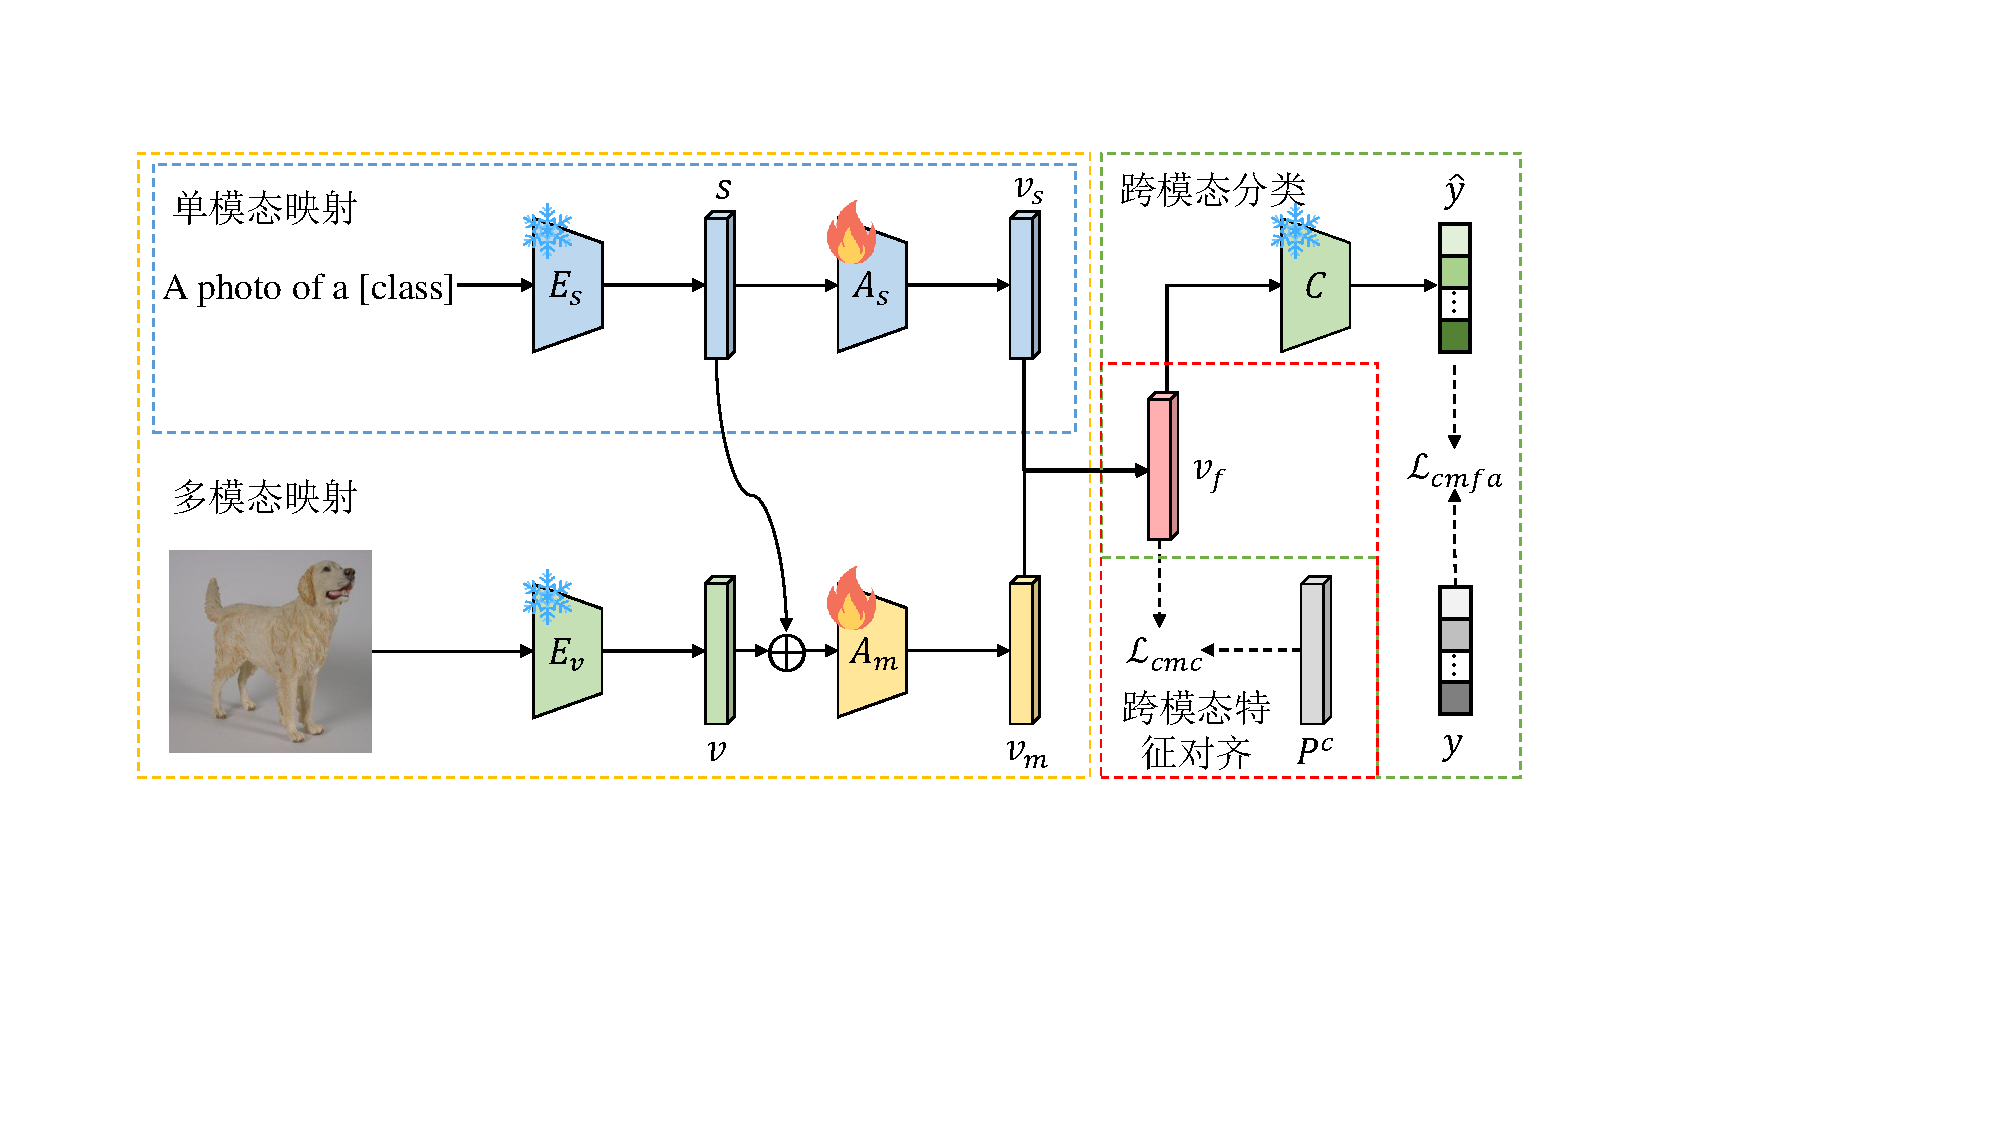
\includegraphics[width=1.0\columnwidth]{figures/SVMSMA/model.pdf}
  % \captionsetup{justification=justified,singlelinecheck=false}
  \bicaption[语义-视觉多空间映射适配模型示意图]{语义-视觉多空间映射适配模型示意图。该模型包含一个视觉特征提取网络$E_v$、一个语义特征提取网络$E_s$,两个语义-视觉多空间映射网络$A_s$与$A_m$,以及一个分类器$C$。在此图中,$v$与$s$分别表示视觉特征与语义特征,$v_s$与$v_m$则是通过$A_s$与$A_m$获得的映射特征,统称为$v_f$。$\widehat{y}$、$y$、$P^c$分别表示预测输出、真实标签和对应类原型特征。$\mathcal{L}_{cmc}$与$\mathcal{L}_{cmfa}$表示跨模态分类损失和跨模态特征对齐损失。另外,模型训练过程中,$E_v$、$E_s$与$C$的参数都被冻结。}[Illustration of Semantic-Visual Multi-Space Mapping Adapter]{Illustration of Semantic-Visual Multi-Space Mapping Adapter. The model includes a visual feature extractor $E_v$, a semantic feature extractor $E_s$, two semantic-visual multi-space mapping networks $A_s$ and $A_m$, and a classifier $C$. In this figure, $v$ and $s$ represent the visual and semantic features, respectively, while $v_s$ and $v_m$ are the mapping features obtained through $A_s$ and $A_m$, collectively referred to as $v_f$. $\widehat{y}$, $y$, and $P^c$ denote the predicted output, true label, and corresponding class prototype features, respectively. $\mathcal{L}_{cmc}$ and $\mathcal{L}_{cmfa}$ represent the cross-modal classification loss and cross-modal feature alignment loss, respectively. Additionally, during the model training process, the parameters of $E_v$, $E_s$, and $C$ are all frozen.}
  \label{figure4: model}
\end{figure}

\subsection[\hspace{-2pt}整体框架]{{\heiti\zihao{4} \hspace{-8pt}整体框架}}\label{section4: 整体框架}

本章提出了一种基于语义-视觉多空间关系建模的少样本特征适配算法,即语义-视觉多空间映射适配模型(Semantic-Visual Multi-Space Mapping Adapter,简称SVMSMA),用以建模样本的语义-视觉多空间关系。该算法旨在利用语义信息作为视觉信息的补充,丰富模型所提取样本特征的信息来源,提升模型在新类上的泛化能力。如图\ref{figure4: model}所示,SVMSMA模型主要包含三个部分:语义-视觉多空间映射网络(Semantic-Visual Multi-Space Mapping Network,简称SVMSMN),跨模态分类(Cross-Modal Classification,简称CMC)模块,以及跨模态特征对齐(Cross-Modal Feature Alignment,简称CMFA)模块。具体来说,语义-视觉多空间映射网络(SVMSMN)用以将语义特征映射到视觉空间,以方便后续与视觉特征进行建模;跨模态分类(CMC)模块通过对映射后的语义特征执行分类任务,以优化映射网络从而使得语义特征与视觉特征建立联系;跨模态特征对齐(CMFA)模块则是将映射后的语义特征与视觉特征原型进行对齐,以对映射后的特征进行修正从而获得更接近类别原型的特征。接下来,本节将会对SVMSMA模型的每个部分进行详细介绍。

\subsection[\hspace{-2pt}语义-视觉多空间映射网络]{{\heiti\zihao{4} \hspace{-8pt}语义-视觉多空间映射网络}}\label{section4: 语义-视觉多空间映射网络}

以方便后续对语义信息与视觉信息进行建模,需要将语义特征和视觉特征投影到相同空间。为了充分利用自然语言处理模型或多模态模型在大规模语料库上对类别名称建立的联系,以及后续建模算法(包括跨模态分类以及跨模态特征对齐)的进行,本文采用将语义特征映射到视觉空间的方式,提出了语义-视觉多空间映射网络(Semantic-Visual Multi-Space Mapping Network,简称SVMSMN),以使得两种信息的特征向量维度一致。本章提出的语义-视觉多空间映射网络可分为两种模式:1)单模态映射,2)多模态映射。这两种模式的核心区别在于它们所处理特征信息的模态种类不同,以下分别对其进行介绍。

\textbf{(1)单模态映射}

单模态映射模式专注于语义信息的处理,其核心思想借鉴了零样本分类领域的思想。该模式的目标是建立一个能够将纯语义信息(例如,文本描述或类别名称)映射至视觉特征空间的高效网络。在实践中,这一过程首先通过语义特征提取网络$E_s$,将类名或提示文本$text$转化为语义特征$s$,
\begin{equation}
  \label{equation4: text to s}
  s = E_s(text).
\end{equation}
随后,单模态映射网络$A_s$负责将这些语义特征映射至视觉空间,生成对应的单模态映射特征$v_s$。该过程可表示为以下公式,
\begin{equation}
  \label{equation4: s to v_s}
  \quad v_s = A_s(s).
\end{equation}

值得注意的是,在本章少样本分类的测试任务中,单模态映射不依赖于任何视觉信息,即不需要支持集的视觉特征参与,这一点使得其更类似于零样本分类的设置。

\textbf{(1)多模态映射}

与单模态映射相比,多模态映射模式采用了一种更为综合和动态的策略,它不仅处理语义信息,同时也将视觉信息作为语义信息的补充。这种模式首先利用预训练的视觉特征提取网络$E_v$,从给定样本图像$x$中提取出丰富的视觉特征$v$,
\begin{equation}
  \label{equation4: x to v}
  v = E_v(x),
\end{equation}
另外通过语义特征提取网络$E_s$获取相应的语义特征$s$,如公式\ref{equation4: text to s}所示。接着,需要对视觉特征和语义特征进行融合,并使用多模态映射网络$A_m$将融合后的多模态特征映射到视觉空间,得到对应的多模态映射特征$v_m$,本章所采用的融合方式为最简单的concat操作。该过程可表达为以下公式,
\begin{equation}
  \label{equation4: v s to v_m}
  v_m = A_m(\text{concat}(v, s)),
\end{equation}

在少样本分类任务中,这种多模态映射模式能够充分利用支持集的视觉特征,以及待分类样本的语义特征,使得所提取特征的信息来源更加丰富,从而更好地适应少样本分类的挑战。

训练过程中,无论是单模态映射模式还是多模态映射模式,SVMSMN都以适配器(Adapter)的方式被插入视觉特征提取网络$E_v$与语义特征提取网络$E_s$之后,视觉特征分类器$C$之前,以在不牺牲特征提取网络泛化能力的前提下,适应本文后续提出的跨模态分类任务和跨模态特征对齐任务。

\subsection[\hspace{-2pt}语义-视觉多空间关系建模算法]{{\heiti\zihao{4} \hspace{-8pt}语义-视觉多空间关系建模算法}}\label{section4: 语义-视觉多空间关系建模算法}

为了建模语义信息和视觉信息的关系,本章提出了两个模块对上一节介绍的语义-视觉多空间映射网络进行优化:1)跨模态分类模块,2)跨模态特征对齐模块。以下将分别对两个模块及其损失进行介绍。

\textbf{(1)跨模态分类}

跨模态分类(Cross-Modal Classification,简称CMC)模块旨在通过分类任务对语义-视觉多空间映射网络进行优化,强化语义信息与视觉信息之间的联系,使得映射后的语义特征能够与实际视觉特征具有一致性。该模块利用预训练视觉特征提取网络时得到的分类器,对通过映射网络得到的单模态或多模态映射特征进行分类,从而促使模型学习到每个类别的语义信息和对应视觉信息之间的紧密对应关系。

具体而言,跨模态分类模块接收映射网络输出的单模态映射特征$v_s$或多模态映射特征$v_m$作为输入,利用分类器$C$计算每个样本的概率分布。该过程可以表达为以下公式,
\begin{equation}
  \label{equation4: softmax}
  \widehat{y} = \text{Softmax}(C(v_f)),
\end{equation}
其中$v_f$表示输入的映射特征,可以为$v_s$或$v_m$,$\widehat{y}$表示样本的预测概率分布。跨模态分类的损失函数采用交叉熵损失,表示为以下公式,
\begin{equation}
  \label{equation4: CMC_loss}
  \mathcal{L}_{cmc} = -\frac{1}{N}\sum_{i=1}^{N}y_i \text{log}\widehat{y}_i,
\end{equation}
其中$N$表示样本数目,$y_i$表示样本类别标签。通过最小化$\mathcal{L}_{cmc}$,模型能够学习到如何将语义信息有效映射到视觉空间,并确保映射后的语义特征与实际类别之间具有高度的一致性。

\textbf{(2)跨模态特征对齐}

跨模态特征对齐(Cross-Modal Feature Alignment,简称CMFA)模块的目的是通过对齐映射特征$v_f$和视觉特征提取网络得到的视觉特征原型$P^c$,以对$v_f$进行修正,使其更接近类别原型,从而提高映射特征$v_f$对每个类别的代表性,进一步提升少样本分类的准确性。

该模块首先计算每个类别的视觉特征原型$P^c$,即该类别所有样本视觉特征的平均值。$P^c$可通过以下公式计算,
\begin{equation}
  \label{equation4: prototype}
  {P}^{c} = \frac{1}{|X^c|} \sum_{i=1}^{|X^c|} v_i,
\end{equation}
其中$X^c$是类别$c$中所有样本的集合,$v_i$是样本$x_i$的视觉特征。接着,CMFA模块计算映射后的视觉特征和对应类别原型之间的距离,并通过最小化该距离来实现特征对齐,该损失函数表示为以下公式,
\begin{equation}
  \label{equation4: CMFA_loss}
  \mathcal{L}_{cmfa} = \frac{1}{N} \sum_{i=1}^{N} || v_{fi} - P^{y_i} ||_2^2,
\end{equation}
其中$|| \cdot ||_2$表示L2范数,用于衡量映射特征$v_{fi}$与对应类别原型$P^{y_i}$之间的欧式距离。通过优化损失函数$\mathcal{L}_{cmfa}$,模型能够引导语义映射特征更贴近于类别的视觉中心,从而获得更具代表性的样本特征,在少样本分类的测试阶段实现更高的准确率。

\subsection[\hspace{-2pt}模型优化]{{\heiti\zihao{4} \hspace{-8pt}模型优化}}\label{section4: 模型优化}

结合公式\ref{equation4: CMC_loss}和\ref{equation4: CMFA_loss},本文提出的SVMSMA模型总体损失函数可以表示为:
\begin{equation}
  \label{equation4: total_loss}
  \mathcal{L}_{total} = \mathcal{L}_{cmc} + \alpha \cdot \mathcal{L}_{cmfa},
\end{equation}
其中,$\alpha$是用来衡量不同损失权重的超参数。

SVMSMA模型在整个基类数据集进行训练,没有采用元学习的方式,并通过最小化损失函数$\mathcal{L}_{total}$对模型参数进行联合优化,通过引入语义信息并对语义-视觉多空间关系进行建模,从而能够丰富模型所获得的信息,更好地迁移在基类数据集上学习到的知识,提升模型的泛化能力。另外,本文中所使用的语义特征提取网络$E_s$基于现有的自然语言处理模型或多模态模型的文本编码器,视觉特征提取网络$E_v$基于使用基类数据集的图像样本预训练的特征提取网络,分类器$C$基于训练视觉特征提取网络时所使用的分类器,$E_s$、$E_v$和$C$的网络参数在本章模型训练时都是冻结的,换句话说,只有单模态映射网络$A_s$和多模态映射网络$A_m$参与了网络参数更新,并且这两个网络是单独进行训练的。

\begin{figure}[h!]
  \centering
  \captionsetup{font={small, stretch=1.312}}
  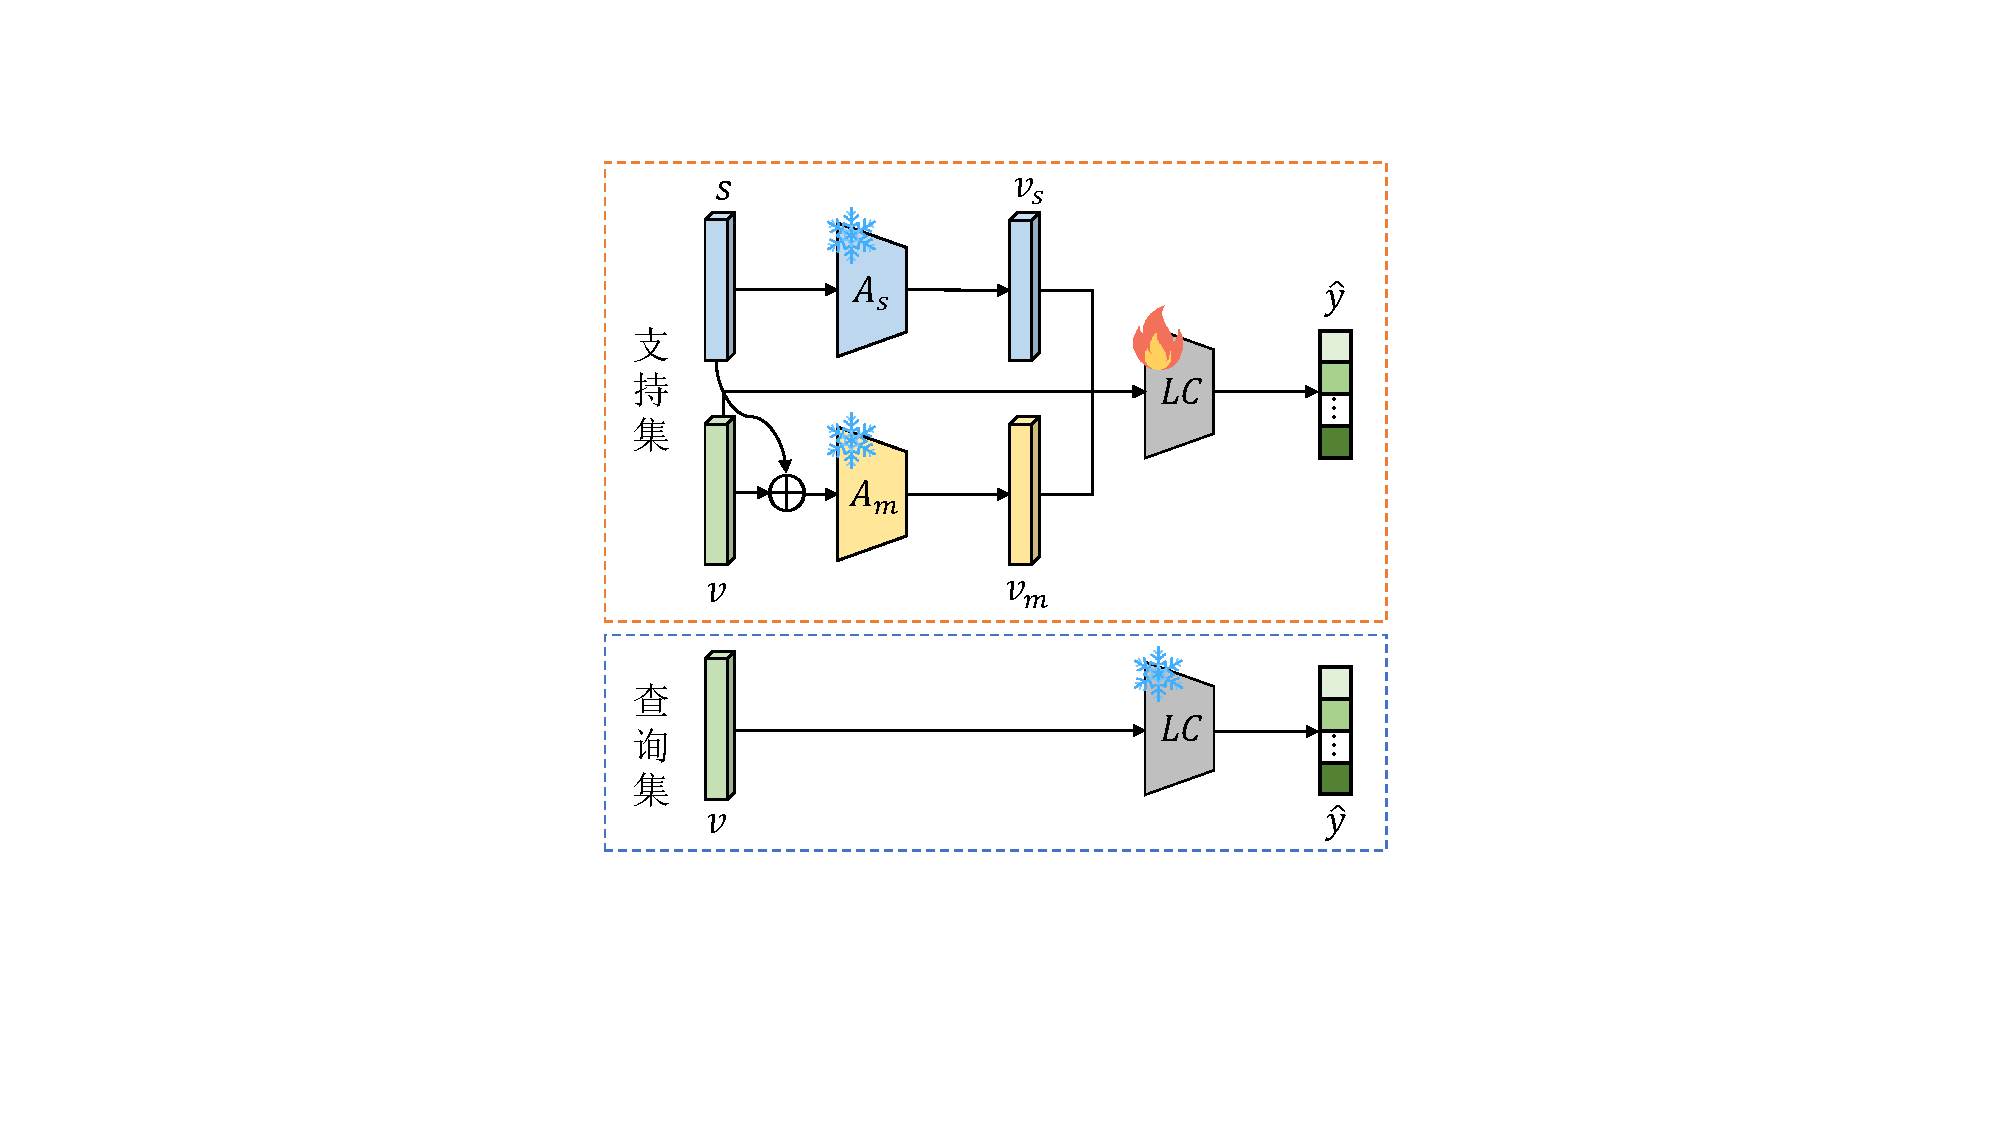
\includegraphics[width=0.6\columnwidth]{figures/SVMSMA/推理过程.pdf}
  % \captionsetup{justification=justified,singlelinecheck=false}
  \bicaption[SVMSMA模型推理过程示意图]{SVMSMA模型推理过程示意图。推理过程中,使用支持集视觉特征$v$、单模态映射特征$v_s$和多模态映射特征$v_m$训练一个逻辑回归分类器$LC$,并使用查询集视觉特征测试分类器性能。}[Illustration of SVMSMA model inference process]{Illustration of SVMSMA model inference process. During the inference process, a logistic regression classifier $LC$ is trained using the visual features $v$, single-modal mapping features $v_s$, and multi-modal mapping features $v_m$ of the support set, and the classifier's performance is tested using the visual features of the query set.}
  \label{figure4: 推理过程}
  \vspace{-7pt}
\end{figure}

\subsection[\hspace{-2pt}模型推理]{{\heiti\zihao{4} \hspace{-8pt}模型推理}}\label{section4: 模型推理}

与第三章相同,本章模型在训练完成之后,在测试阶段同样冻结所有模型参数并通过使用逻辑回归分类器$LC$执行多个少样本分类任务,将平均准确率作为模型的评价指标。不同的是,每个任务的推理过程中,本章会使用单模态映射网络$A_s$以及多模态映射网络$A_m$得到的语义映射特征$v_s$和$v_m$对原本支持集$\mathcal{S}_{\mathcal{T}}$的视觉特征$v$进行扩充,以丰富支持集样本特征的信息来源及其多样性,从而使分类器学习到更好的分类边界,达到更好的分类性能。与生成方法经常扩充支持集样本至原来的几十倍甚至上百倍不同,本文方法仅将支持集样本特征扩充至原来的3倍。对于查询集,由于无法获得其类别名称(获得类别名称相当于已知其类别),则是将其视觉特征输入训练完成的分类器$LC$获得其预测类别。本章模型推理过程如图\ref{figure4: 推理过程}所示。

\section[\hspace{-2pt}实验设置及结果分析]{{\heiti\zihao{-3} \hspace{-8pt}实验设置及结果分析}}\label{section4: 实验设置及结果分析}

在本节中,首先介绍了本章方法的实验设置,包括实验使用数据集、网络结构、以及优化设置,然后分析了基于语义-视觉多空间关系建模的少样本特征适配算法实验结果,接下来对模型的各个模块以及超参数进行了消融实验和分析,最后对模型所提取特征进行了可视化分析。

\subsection[\hspace{-2pt}实验设置]{{\heiti\zihao{4} \hspace{-8pt}实验设置}}\label{section4: 实验设置}

\textbf{(1)实验数据集介绍}

与第三章相同,本章方法同样在四个少样本分类基准数据集进行了实验,包括三个普通少样本分类数据集:miniImageNet \cite{vinyals2016matching}、tieredImageNet \cite{ren2018meta}、CIFAR-FS \cite{bertinetto2019meta},以及一个细粒度少样本分类数据集:CUB-200-2011(CUB)\cite{wah2011caltech}。不同的是,第三章方法仅使用了数据集中每个样本的图像以及标签,而本章方法还使用了数据集中包含的样本类别名称来提供语义信息。

\textbf{(2)网络结构}

在没有特殊说明的情况下,本文所使用视觉特征提取网络为第三章MGSRCL模型的特征提取网络,语义特征提取网络与SP-CLIP\cite{SP-CLIP}相同,为使用ViT-B/16架构作为图像编码器的CLIP模型的文本编码器,其输出语义特征维度为512。并且在使用CLIP模型获取语义特征时,本章方法使用了基于提示的方法,将提示文本“A photo of a”与类别名称“[class]”拼接后作为输入,如图\ref{figure4: model}所示。语义-视觉多空间映射网络则是由两层全连接,和处于两层全连接之间的ReLU激活函数组成的多层感知机。输入层维度为语义特征维度(单模态映射)或视觉特征维度和语义特征维度之和(多模态映射),隐藏层维度为4096,输出层维度为视觉特征维度。

\textbf{(3)优化设置}

对于所有实验,本文采用具有5$e^{-4}$权重衰减的自适应矩估计(Adaptive Moment Estimation,简称Adam)优化器对模型进行优化,对于tieredImageNet数据集,学习率设置为1$e^{-4}$,其余数据集均设置为1$e^{-5}$,对于所有数据集均训练100个轮次。在训练过程中,视觉特征提取网络$E_v$、语义特征提取网络$E_s$、分类器$C$参数均被冻结,只有单模态映射网络$A_s$或多模态映射网络$A_m$参与参数更新。对于超参数$\alpha$,本文在CIFAR-FS数据集将其设置为10.0,其他数据集均设置为1.0,超参数讨论将在\ref{section4: 消融实验}部分进行。

\subsection[\hspace{-2pt}基准数据集实验结果]{{\heiti\zihao{4} \hspace{-8pt}基准数据集实验结果}}\label{section4: 基准数据集实验结果}

为了评估SVMSMA模型的有效性,本文在四个数据集上进行了大量实验。模型评估过程中,同样对5-way 1-shot以及5-way 5-shot分别采样2000个任务并计算平均分类准确率作为最终实验结果。表\ref{table4: mini}、\ref{table4: tiered}、\ref{table4: CIFAR-FS}和\ref{table4: CUB}分别展示了本章方法在miniImageNet、tieredImageNet、CIFAR-FS和CUB数据集上的实验结果以及一些其他现有少样本分类方法的结果。

\textbf{(1)普通少样本分类}

与其他少样本方法相比较,本章方法SVMSMA在miniImageNet、CIFAR-FS数据集达到了最优结果,在tieredImageNet数据集达到了第二优结果,如表\ref{table4: mini}、\ref{table4: tiered}和\ref{table4: CIFAR-FS}所示。具体而言,本章提出的SVMSMA模型在miniImageNet数据集上的5-way 1-shot和5-way 5-shot任务分别达到了79.58\%和85.19\%的准确率,与第二优方法相比分别高出了7.27\%和0.79\%。在CIFAR-FS数据集,SVMSMA模型在1-shot和5-shot任务则是分别达到了86.35\%和89.42\%的准确率,比分别在1-shot和5-shot任务上达到次优结果的SP-CLIP和IER方法高出了4.17\%和0.16\%。在tieredImageNet数据集,则是SP-CLIP方法达到了最优结果,本章方法达到了第二优结果,1-shot与5-shot任务准确率分别是75.35\%和86.35\%。这些实验结果证明了本章方法的有效性。

{
\small    % 设置表格字体为5号
\setstretch{1.245}        % 设置具有指定弹力的橡皮长度(原行宽的1.2倍)
\captionsetup{font={small, stretch=1.512}}
\begin{xltabular}{\textwidth}{Clccc}
  \bilingualcaption{SVMSMA在miniImageNet数据集上的分类准确率(\%)}{SVMSMA在miniImageNet数据集上的分类准确率(\%)。最优结果用粗体表示,“Visual”与“Semantic”分别表示没有使用语义信息的方法与基于语义的方法。}{Classification accuracy (\%) of SVMSMA on miniImageNet. The best results are shown in bold, ``Visual'' and ``Semantic'' respectively refer to methods without the use of semantic information and methods based on semantic information.}
  \label{table4: mini} \\
  \toprule
  & 方法 & 特征提取网络 & 5-way 1-shot & 5-way 5-shot \\
  \midrule
  \endfirsthead

  \multicolumn{5}{c}{\tablename \thetable{} (续)} \\ % 第一行标题
  \multicolumn{5}{c}{Table \thetable{} (continued)} \\ % 第二行标题

  \toprule
  & 方法 & 特征提取网络 & 5-way 1-shot & 5-way 5-shot \\
  \midrule
  \endhead

  % \midrule \multicolumn{3}{r}{{接下页}} \\ 
  \bottomrule
  \endfoot

  \bottomrule
  \endlastfoot

  % 添加你的内容
  \multirow{14}{*}{Visual}
  & MAML \cite{MAML} & 32-32-32-32 & 48.70 $\pm$ 1.84 & 63.11 $\pm$ 0.92 \\
  & ProtoNet \cite{ProtoNet} & 64-64-64-64 & $ 49.42 \pm 0.78 $ & 68.20 $\pm$ 0.66 \\
  & DeepEMD \cite{DeepEMD} & ResNet-12 & 65.91 $\pm$ 0.82 & 82.41 $\pm$ 0.56 \\
  & RFS-distill \cite{RFS} & ResNet-12 & 64.82 $\pm$ 0.60 & 82.14 $\pm$ 0.43 \\
  % \multirow{15}{*}{Visual}
  & AssoAlign \cite{AssoAlign} & ResNet-18 & 59.88 $\pm$ 0.67 & 80.35 $\pm$ 0.73 \\
  & FEAT \cite{FEAT} & ResNet-12 & 66.78 $\pm$ 0.20 & 82.05 $\pm$ 0.14 \\
  & GIFSL \cite{GIFSL} & ResNet-12 & 65.47 $\pm$ 0.63 & 82.75 $\pm$ 0.42 \\
  & MELR \cite{MELR} & ResNet-12 & 67.40 $\pm$ 0.43 & 83.40 $\pm$ 0.28\\
  & IEPT \cite{IEPT} & ResNet-12 & 67.05 $\pm$ 0.44 & 82.90 $\pm$ 0.30 \\
  & IER \cite{IER} & ResNet-12 & 66.82 $\pm$ 0.80 & 84.35 $\pm$ 0.51 \\
  & RENet \cite{RENet} & ResNet-12 & 67.60 $\pm$ 0.44 & 82.58 $\pm$ 0.30 \\
  & PAL \cite{PAL} & ResNet-12 & 69.37 $\pm$ 0.64 & 84.40 $\pm$ 0.44 \\
  & HandCrafted \cite{HandCrafted} & ResNet-12 & 67.14 $\pm$ 0.76 & 83.11 $\pm$ 0.69 \\
  & SCL-distill \cite{Spatial} & ResNet-12 & 67.40 $\pm$ 0.76 & 83.19 $\pm$ 0.54 \\
  \multirow{8}{*}{Visual}
  & HGNN \cite{HGNN} & ResNet-12 & 67.02 $\pm$ 0.20 & 83.00 $\pm$ 0.13 \\
  & APP2S \cite{APP2S} & ResNet-18 & 64.82 $\pm$ 0.12 & 81.31 $\pm$ 0.22 \\
  & ESPT \cite{ESPT} & ResNet-12 & 68.36 $\pm$ 0.19 & 84.11 $\pm$ 0.12 \\
  & Meta-HP \cite{Meta-HP} & ResNet-12 & 62.49 $\pm$ 0.80 & 77.12 $\pm$ 0.62 \\
  & SAPENet \cite{SAPENet} & ResNet-12 & 66.41 $\pm$ 0.20 & 82.76 $\pm$ 0.14 \\
  & FEAT+DFR \cite{DFR} & ResNet-12 & 67.74 $\pm$ 0.86 & 82.49 $\pm$ 0.57 \\
  & DiffKendall \cite{DiffKendall} & ResNet-12 & 65.56 $\pm$ 0.43 & 80.79 $\pm$ 0.31 \\
  % & FGFL \cite{FGFL} & ResNet-12 & 69.14 $\pm$ 0.80 & 86.01 $\pm$ 0.62 \\
  & MetaDiff \cite{MetaDiff} & ResNet-12 & 64.99 $\pm$ 0.77 & 81.21 $\pm$ 0.56 \\
  \midrule
  \multirow{9}{*}{Semantic}
  & KTN \cite{KTN} & 64-64-128-128 & 64.42 $\pm$ 0.72 & 74.16 $\pm$ 0.56 \\
  & DualTriNet \cite{DualTriNet} & ResNet-18 & 58.12 $\pm$ 1.37 & 76.92 $\pm$ 0.69 \\
  & AM3 \cite{AM3} & ResNet-12 & 65.30 $\pm$ 0.49 & 78.10 $\pm$ 0.36 \\
  & TRAML \cite{TRAML} & ResNet-12 & 67.10 $\pm$ 0.52 & 79.54 $\pm$ 0.60 \\
  & AM3-BERT \cite{yan2021aligning} & ResNet-12 & 68.42 $\pm$ 0.51 & 81.29 $\pm$ 0.59 \\
  & CMGNN-DPGN \cite{CMGNN-DPGN} & ResNet-12 & 71.38 $\pm$ 0.51 & 82.60 $\pm$ 0.47 \\
  & STVAE \cite{STVAE} & ResNet-12 & 63.62 $\pm$ 0.80 & 80.68 $\pm$ 0.48 \\
  & SP-CLIP \cite{SP-CLIP} & Visformer-T & 72.31 $\pm$ 0.40 & 83.42 $\pm$ 0.30 \\
  \cline{2-5}
  & \raisebox{-2pt}{\textbf{SVMSMA}} & \raisebox{-2pt}{ResNet-12} & \raisebox{-2pt}{\textbf{79.58 $\pm$ 0.35}} & \raisebox{-2pt}{\textbf{85.19 $\pm$ 0.29}} \\
\end{xltabular}}


{
\small    % 设置表格字体为5号
\setstretch{1.245}        % 设置具有指定弹力的橡皮长度(原行宽的1.2倍)
\captionsetup{font={small, stretch=1.512}}
\begin{xltabular}{\textwidth}{Clccc}
  \bilingualcaption{SVMSMA在tieredImageNet数据集上的分类准确率(\%)}{SVMSMA在tieredImageNet数据集上的分类准确率(\%)。最优结果用粗体表示,带有“\dag”标记的方法表示结果是使用作者提供代码所实现,“Visual”与“Semantic”分别表示没有使用语义信息的方法与基于语义的方法。}{Classification accuracy (\%) of SVMSMA on tieredImageNet. The best results are shown in bold, and methods with the ``\dag'' indicate that the result was implemented using author-supplied code, ``Visual'' and ``Semantic'' respectively refer to methods without the use of semantic information and methods based on semantic information.}
  \label{table4: tiered} \\
  \toprule
  & 方法 & 特征提取网络 & 5-way 1-shot & 5-way 5-shot \\
  \midrule
  \endfirsthead

  \multicolumn{5}{c}{\tablename \thetable{} (续)} \\ % 第一行标题
  \multicolumn{5}{c}{Table \thetable{} (continued)} \\ % 第二行标题

  \toprule
  & 方法 & 特征提取网络 & 5-way 1-shot & 5-way 5-shot \\
  \midrule
  \endhead

  % \midrule \multicolumn{3}{r}{{接下页}} \\ 
  \bottomrule
  \endfoot

  \bottomrule
  \endlastfoot

  % 添加你的内容
  \multirow{10}{*}{Visual}
  & MAML \cite{MAML} & 32-32-32-32 & 51.67 $\pm$ 1.81 & 70.30 $\pm$ 1.75 \\
  & ProtoNet \cite{ProtoNet} & 64-64-64-64  & 53.31 $\pm$ 0.89 & 72.69 $\pm$ 0.74 \\
  & DeepEMD \cite{DeepEMD} & ResNet-12 & 71.16 $\pm$ 0.87 & 86.03 $\pm$ 0.58 \\
  & RFS-distill \cite{RFS} & ResNet-12 & 71.52 $\pm$ 0.69 & 86.03 $\pm$ 0.49 \\
  & AssoAlign \cite{AssoAlign} & ResNet-18 & 69.29 $\pm$ 0.56 & 85.97 $\pm$ 0.49 \\
  & FEAT \cite{FEAT} & ResNet-12 & 70.80 $\pm$ 0.23 & 84.79 $\pm$ 0.16 \\
  & GIFSL \cite{GIFSL} & ResNet-12 & 72.39 $\pm$ 0.66 & 86.91 $\pm$ 0.44 \\
  & MELR \cite{MELR} & ResNet-12 & 72.14 $\pm$ 0.51 & 87.01 $\pm$ 0.35 \\
  & IEPT \cite{IEPT} & ResNet-12 & 72.24 $\pm$ 0.50 & 86.73 $\pm$ 0.34 \\
  & IER \cite{IER} & ResNet-12 & 71.87 $\pm$ 0.89 & 86.82 $\pm$ 0.58 \\
  \multirow{11}{*}{Visual}
  & RENet \cite{RENet} & ResNet-12 & 71.16 $\pm$ 0.51 & 85.28 $\pm$ 0.35 \\
  & PAL \cite{PAL} & ResNet-12 & 72.25 $\pm$ 0.72 & 86.95 $\pm$ 0.47 \\
  & SCL-distill \cite{Spatial} & ResNet-12 & 71.98 $\pm$ 0.91 & 86.19 $\pm$ 0.59 \\
  & HGNN \cite{HGNN} & ResNet-12 & 72.05 $\pm$ 0.23 & 86.49 $\pm$ 0.15 \\
  & APP2S \cite{APP2S} & ResNet-18 & 70.83 $\pm$ 0.15 & 84.15 $\pm$ 0.29 \\
  & ESPT \cite{ESPT} & ResNet-12 & 72.68 $\pm$ 0.22 & 87.49 $\pm$ 0.14 \\
  & Meta-HP \cite{Meta-HP} & ResNet-12 & 68.26 $\pm$ 0.72 & 82.91 $\pm$ 0.36 \\
  & SAPENet \cite{SAPENet} & ResNet-12 & 68.63 $\pm$ 0.23 & 84.30 $\pm$ 0.16 \\
  & FEAT+DFR \cite{DFR} & ResNet-12 & 71.31 $\pm$ 0.93 & 85.12 $\pm$ 0.64 \\
  & DiffKendall \cite{DiffKendall} & ResNet-12 & 70.76 $\pm$ 0.43 & 85.31 $\pm$ 0.34 \\
  % & FGFL \cite{FGFL} & ResNet-12 & 73.21 $\pm$ 0.88 & 87.21 $\pm$ 0.61 \\
  & MetaDiff \cite{MetaDiff} & ResNet-12 & 72.33 $\pm$ 0.92 & 86.31 $\pm$ 0.62 \\
  \midrule
  \multirow{6}{*}{Semantic}
  & AM3 \cite{AM3} & ResNet-12 & 69.08 $\pm$ 0.47 & 82.58 $\pm$ 0.31 \\
  & AM3-BERT \cite{yan2021aligning} & ResNet-12 & 73.76 $\pm$ 0.72 & 87.51 $\pm$ 0.75 \\
  & CMGNN-DPGN \cite{CMGNN-DPGN} & ResNet-12 & 72.89 $\pm$ 0.49 & 84.92 $\pm$ 0.48 \\
  & STVAE\dag \cite{STVAE} & ResNet-12 & 68.32 $\pm$ 0.94 & 83.79 $\pm$ 0.66 \\
  & SP-CLIP \cite{SP-CLIP} & Visformer-T & \textbf{78.03 $\pm$ 0.46} & \textbf{88.55 $\pm$ 0.32} \\
  \cline{2-5}
  & \raisebox{-2pt}{\textbf{SVMSMA}} & \raisebox{-2pt}{ResNet-12} & \raisebox{-2pt}{75.35 $\pm$ 0.47} & \raisebox{-2pt}{86.35 $\pm$ 0.34} \\
\end{xltabular}}

{
\small    % 设置表格字体为5号
\setstretch{1.245}        % 设置具有指定弹力的橡皮长度(原行宽的1.2倍)
\captionsetup{font={small, stretch=1.512}}
\begin{xltabular}{\textwidth}{Clccc}
  \bilingualcaption{SVMSMA在CIFAR-FS数据集上的分类准确率(\%)}{SVMSMA在CIFAR-FS数据集上的分类准确率(\%)。最优结果用粗体表示,“Visual”与“Semantic”分别表示没有使用语义信息的方法与基于语义的方法。}{Classification accuracy (\%) of SVMSMA on CIFAR-FS. The best results are shown in bold, ``Visual'' and ``Semantic'' respectively refer to methods without the use of semantic information and methods based on semantic information.}
  \label{table4: CIFAR-FS} \\
  \toprule
  & 方法 & 特征提取网络 & 5-way 1-shot & 5-way 5-shot \\
  \midrule
  \endfirsthead

  \multicolumn{5}{c}{\tablename \thetable{} (续)} \\ % 第一行标题
  \multicolumn{5}{c}{Table \thetable{} (continued)} \\ % 第二行标题

  \toprule
  & 方法 & 特征提取网络 & 5-way 1-shot & 5-way 5-shot \\
  \midrule
  \endhead

  % \midrule \multicolumn{3}{r}{{接下页}} \\ 
  \bottomrule
  \endfoot

  \bottomrule
  \endlastfoot

  % 添加你的内容
  \multirow{12}{*}{Visual}
  & MAML \cite{MAML} & 32-32-32-32 & 58.90 $\pm$ 1.90 & 71.50 $\pm$ 1.00 \\
  & ProtoNet \cite{ProtoNet} & 64-64-64-64 & 55.50 $\pm$ 0.70 & 72.00 $\pm$ 0.60 \\
  & RFS-distill \cite{RFS} & ResNet-12 & 73.90 $\pm$ 0.80 & 86.90 $\pm$ 0.50  \\
  & GIFSL \cite{GIFSL} & ResNet-12 & 74.58 $\pm$ 0.38 & 87.68 $\pm$ 0.23 \\
  & IER \cite{IER} & ResNet-12 & 76.83 $\pm$ 0.82 & 89.26 $\pm$ 0.58  \\
  & RENet \cite{RENet} & ResNet-12 & 74.51 $\pm$ 0.46 & 86.60 $\pm$ 0.32  \\
  & PAL \cite{PAL} & ResNet-12 & 77.10 $\pm$ 0.70 & 88.00 $\pm$ 0.50  \\
  & HandCrafted \cite{HandCrafted} & ResNet-12 & 76.68 $\pm$ 0.59 & 87.49 $\pm$ 0.73 \\
  & SCL-distill \cite{Spatial} & ResNet-12 & 76.50 $\pm$ 0.90 & 88.00 $\pm$ 0.60  \\
  & ConstellationNet \cite{ConstellationNet} & ResNet-12 & 75.40 $\pm$ 0.20 & 86.80 $\pm$ 0.20  \\
  & APP2S \cite{APP2S} & ResNet-18 & 73.12 $\pm$ 0.22 & 85.69 $\pm$ 0.16 \\
  & Meta-HP \cite{Meta-HP} & ResNet-12 & 73.74 $\pm$ 0.57 & 86.37 $\pm$ 0.32 \\
  \midrule
  \multirow{4}{*}{Semantic}
  & DualTriNet \cite{DualTriNet} & ResNet-18 & 63.41 $\pm$ 0.64 & 78.43 $\pm$ 0.62 \\
  & STVAE \cite{STVAE} & ResNet-12 & 76.30 $\pm$ 0.60 & 87.00 $\pm$ 0.40 \\
  & SP-CLIP \cite{SP-CLIP} & Visformer-T & 82.18 $\pm$ 0.40 & 88.24 $\pm$ 0.32 \\
  \cline{2-5}
  & \raisebox{-2pt}{\textbf{SVMSMA}} & \raisebox{-2pt}{ResNet-12} & \raisebox{-2pt}{\textbf{86.35 $\pm$ 0.35}} & \raisebox{-2pt}{\textbf{89.42 $\pm$ 0.30}} \\
\end{xltabular}}

\textbf{(2)细粒度少样本分类}

同样的,本章方法也在细粒度少样本分类数据集CUB上进行了实验,结果如表\ref{table4: CUB}所示。在CUB数据集,SVMSMA模型同样取得了最优结果,在1-shot和5-shot任务上分别达到了91.17\%和94.91\%的平均准确率,比第二优的方法分别高出了5.72\%和0.18\%。这一实验证明了在类别差异较小的细粒度数据集,语义信息同样能够为视觉信息提供帮助,获得进一步性能提升。

{
\small    % 设置表格字体为5号
\setstretch{1.245}        % 设置具有指定弹力的橡皮长度(原行宽的1.2倍)
\captionsetup{font={small, stretch=1.512}}
\begin{xltabular}{\textwidth}{Clccc}
  \bilingualcaption{SVMSMA在CUB数据集上的分类准确率(\%)}{SVMSMA在CUB数据集上的分类准确率(\%)。最优结果用粗体表示,“Visual”与“Semantic”分别表示没有使用语义信息的方法与基于语义的方法。}{Classification accuracy (\%) of SVMSMA on CUB. The best results are shown in bold, ``Visual'' and ``Semantic'' respectively refer to methods without the use of semantic information and methods based on semantic information.}
  \label{table4: CUB} \\
  \toprule
  & 方法 & 特征提取网络 & 5-way 1-shot & 5-way 5-shot \\
  \midrule
  \endfirsthead

  \multicolumn{5}{c}{\tablename \thetable{} (续)} \\ % 第一行标题
  \multicolumn{5}{c}{Table \thetable{} (continued)} \\ % 第二行标题

  \toprule
  & 方法 & 特征提取网络 & 5-way 1-shot & 5-way 5-shot \\
  \midrule
  \endhead

  % \midrule \multicolumn{3}{r}{{接下页}} \\ 
  \bottomrule
  \endfoot

  \bottomrule
  \endlastfoot

  % 添加你的内容
  \multirow{12}{*}{Visual}
  % \multirow{7}{*}{Visual}
  & FEAT \cite{FEAT} & 64-64-64-64 & 68.87 $\pm$ 0.22 & 82.90 $\pm$ 0.15 \\
  & DeepEMD \cite{DeepEMD} & ResNet-12 & 75.65 $\pm$ 0.83 & 88.69 $\pm$ 0.50 \\
  & AssoAlign \cite{AssoAlign} & ResNet-18 & 74.22 $\pm$ 1.09 & 88.65 $\pm$ 0.55 \\
  & MELR \cite{MELR} & 64-64-64-64 & 70.26 $\pm$ 0.50 & 85.01 $\pm$ 0.32 \\
  & IEPT \cite{IEPT} & 64-64-64-64 & 69.97 $\pm$ 0.49 & 84.33 $\pm$ 0.33 \\
  & RENet \cite{RENet} & ResNet-12 & 79.49 $\pm$ 0.44 & 91.11 $\pm$ 0.24 \\
  & HGNN \cite{HGNN} & ResNet-12 & 78.58 $\pm$ 0.20 & 90.02 $\pm$ 0.12 \\
  & APP2S \cite{APP2S} & ResNet-12 & 77.64 $\pm$ 0.19 & 90.43 $\pm$ 0.18 \\
  & ESPT \cite{ESPT} & ResNet-12 & 85.45 $\pm$ 0.18 & 94.02 $\pm$ 0.09 \\
  & SAPENet \cite{SAPENet} & 64-64-64-64 & 70.38 $\pm$ 0.23 & 84.47 $\pm$ 0.14 \\
  & FEAT+DFR \cite{DFR} & ResNet-12 & 77.14 $\pm$ 0.21 & 88.97 $\pm$ 0.13 \\
  % & FGFL \cite{FGFL} & ResNet-12 & 80.77 $\pm$ 0.90 & 92.01 $\pm$ 0.71 \\
  & Bi-FRN \cite{Bi-FRN} & ResNet-12 & 85.44 $\pm$ 0.18 & 94.73 $\pm$ 0.09 \\
  \midrule
  \multirow{4}{*}{Semantic}
  & DualTriNet \cite{DualTriNet} & ResNet-18 & 69.61 $\pm$ 0.46 & 84.10 $\pm$ 0.35 \\
  & AM3-BERT \cite{yan2021aligning} & ResNet-12 & 77.03 $\pm$ 0.85 & 87.20 $\pm$ 0.70 \\
  & STVAE \cite{STVAE} & ResNet-12 & 77.32 $\pm$ 0.00 & 86.84 $\pm$ 0.00 \\
  \cline{2-5}
  & \raisebox{-2pt}{\textbf{SVMSMA}} & \raisebox{-2pt}{ResNet-12} & \raisebox{-2pt}{\textbf{91.17 $\pm$ 0.28}} & \raisebox{-2pt}{\textbf{94.91 $\pm$ 0.19}} \\
\end{xltabular}}

综上所述,本章提出的SVMSMA方法在miniImageNet、CIFAR-FS和CUB三个数据集达到了最优结果,在tieredImageNet数据集也达到了第二优结果,这证明了SVMSMA模型通过引入语义信息对视觉信息进行补充,使得样本特征信息来源更加丰富,从而获得更具代表性和多样性的特征,提升模型的泛化能力。另外,相比于5-way 5-shot任务,SVMSMA模型在5-way 1-shot任务取得了更为明显的效果提升,这是因为5-shot任务样本多样性已较为充足,能够使得分类器从中提取到样本关键特征进行分类,而1-shot任务样本数量较少,不足以训练一个具有良好分类边界的分类器,使用语义特征可对视觉特征进行补充,提升特征多样性,优化分类边界。

\textbf{(3)与SP-CLIP方法对比}

针对在tieredImageNet数据集上本文方法SVMSMA较SP-CLIP方法差的现象,本文猜测可能是由于SP-CLIP方法预训练网络基于Transformer架构,并且图像分辨率为224 $\times$ 244,而SVMSMA使用的预训练模型基于卷积网络架构,且图像分辨率为84 $\times$ 84。由于Transformer模型中的自注意力机制在数据集规模较大时能够更好地捕获全局信息,使其达到较卷积网络更好的结果,导致SP-CLIP在tieredImageNet数据集上能够达到更好的效果。为了验证此观点,本文使用SP-CLIP的预训练网络作为视觉特征提取网络在miniImageNet、tieredImageNet、CIFAR-FS数据集上进行了进一步实验,以在相同视觉特征提取网络与语义特征提取网络的条件下公平对比本文方法与SP-CLIP方法。

\begin{table}[h!]
  \small    % 设置表格字体为5号
  \setstretch{1.245}        % 设置具有指定弹力的橡皮长度(原行宽的1.2倍)
  \captionsetup{font={small, stretch=1.512}}
  \centering
  % \vspace{-10pt}
  \bicaption[SVMSMA与SP-CLIP的对比实验]{SVMSMA与SP-CLIP的对比实验。最优结果用粗体表示。}{Comparison of SVMSMA and SP-CLIP. The best results are shown in bold.}    % 中英文标题
  \begin{tabularx}{\textwidth}{ClCCC}
    \toprule
    数据集 & 方法      & 特征提取网络      & 5-way 1-shot              & 5-way 5-shot              \\
    \midrule
    \multirow{3}*{miniImageNet}
        & SP-CLIP & Visformer-T & 72.31 $\pm$ 0.40          & 83.42 $\pm$ 0.30          \\
        & SVMSMA  & Visformer-T & 73.51 $\pm$ 0.38          & 83.29 $\pm$ 0.32          \\
        & SVMSMA  & ResNet-12   & \textbf{79.58 $\pm$ 0.35} & \textbf{85.19 $\pm$ 0.29} \\
    \midrule
    \multirow{3}*{tieredImageNet}
        & SP-CLIP & Visformer-T & 78.03 $\pm$ 0.46          & 88.55 $\pm$ 0.32          \\
        & SVMSMA  & Visformer-T & \textbf{79.48 $\pm$ 0.44} & \textbf{88.59 $\pm$ 0.32} \\
        & SVMSMA  & ResNet-12   & 75.35 $\pm$ 0.47          & 86.35 $\pm$ 0.34          \\
    \midrule
    \multirow{3}*{CIFAR-FS}
        & SP-CLIP & Visformer-T & 82.18 $\pm$ 0.40          & 88.24 $\pm$ 0.32          \\
        & SVMSMA  & Visformer-T & 82.44 $\pm$ 0.38          & 88.32 $\pm$ 0.33          \\
        & SVMSMA  & ResNet-12   & \textbf{86.35 $\pm$ 0.35} & \textbf{89.42 $\pm$ 0.30} \\
    \bottomrule
  \end{tabularx}
  % \vspace{-25pt}
  \label{table4: comparison with SP}
\end{table}

此部分实验比较共包含三个模型,分别是SP-CLIP、使用SP-CLIP预训练网络作为视觉特征提取网络的SVMSMA(Visformer-T)、以及使用上章方法MGSRCL作为视觉特征提取网络的SVMSMA(ResNet-12),如表\ref{table4: comparison with SP}所示。实验结果显示,在5-way 1-shot任务上,SVMSMA(Visformer-T)在三个数据集上都达到了较SP-CLIP方法高的分类准确率,在miniImageNet、tieredImageNet、CIFAR-FS数据集上分别取得了1.20\%、1.45\%和0.26\%的性能提升。在5-way 5-shot任务也达到了和SP-CLIP方法相当的性能表现,仅在miniImageNet数据集准确率略微下降。这些实验结果证明了本文方法通过简单的映射网络以及损失设计便可有效利用语义信息,提升少样本分类准确率。另外,可以观察到,使用MGSRCL作为视觉特征提取网络的模型在miniImageNet、CIFAR-FS两个数据集取得了最优结果,这一现象进一步说明了第三章提到的特征学习阶段对于少样本分类的重要性。

\subsection[\hspace{-2pt}消融实验]{{\heiti\zihao{4} \hspace{-8pt}消融实验}}\label{section4: 消融实验}

\textbf{(1)讨论不同模块对模型性能的影响}

为了研究SVMSMA模型中每个模块对模型的影响,本文在miniImageNet、CIFAR-FS和CUB三个数据集上进行了消融实验,此部分实验分为四个模型,分别为基准模型(Baseline),添加跨模态分类(CMC)模块的基准模型(Baseline w/ CMC),添加跨模态特征对齐(CMFA)模块的基准模型(Baseline w/ CMFA),以及最终模型SVMSMA。此处的基准模型(Baseline)为上一章仅使用视觉信息的多粒度样本关系对比学习(MGSRCL)模型。

\begin{table}[h!]
  \small    % 设置表格字体为5号
  \setstretch{1.245}        % 设置具有指定弹力的橡皮长度(原行宽的1.2倍)
  \captionsetup{font={small, stretch=1.512}}
  \centering
  % \vspace{-10pt}
  \bicaption[SVMSMA在miniImageNet、CIFAR-FS和CUB数据集上的模块消融实验]{SVMSMA在miniImageNet、CIFAR-FS和CUB数据集上的模块消融实验。最优结果用粗体表示。}{Module ablation experiments of SVMSMA on miniImageNet, CIFAR-FS and CUB. The best results are shown in bold.}    % 中英文标题
  \begin{tabularx}{\textwidth}{ClCC}
    \toprule
    数据集 & 方法               & 5-way 1-shot              & 5-way 5-shot              \\
    \midrule
    \multirow{4}{*}{miniImageNet}
        & Baseline         & 69.57 $\pm$ 0.45          & 84.41 $\pm$ 0.30          \\
        & Baseline w/ CMC  & 76.41 $\pm$ 0.39          & 84.74 $\pm$ 0.29          \\
        & Baseline w/ CMFA & 78.82 $\pm$ 0.36          & 84.82 $\pm$ 0.29          \\
        & SVMSMA           & \textbf{79.58 $\pm$ 0.35} & \textbf{85.19 $\pm$ 0.29} \\
    \midrule
    \multirow{4}{*}{CIFAR-FS}
        & Baseline         & 78.54 $\pm$ 0.47          & 88.64 $\pm$ 0.32          \\
        & Baseline w/ CMC  & 84.18 $\pm$ 0.39          & 89.12 $\pm$ 0.31          \\
        & Baseline w/ CMFA & 85.31 $\pm$ 0.38          & 89.18 $\pm$ 0.31          \\
        & SVMSMA           & \textbf{86.35 $\pm$ 0.35} & \textbf{89.42 $\pm$ 0.30} \\
    \midrule
    \multirow{4}{*}{CUB}
        & Baseline         & 86.14 $\pm$ 0.38          & 94.75 $\pm$ 0.19          \\
        & Baseline w/ CMC  & 90.20 $\pm$ 0.30          & 94.65 $\pm$ 0.19          \\
        & Baseline w/ CMFA & 91.02 $\pm$ 0.29          & 94.65 $\pm$ 0.19          \\
        & SVMSMA           & \textbf{91.17 $\pm$ 0.28} & \textbf{94.91 $\pm$ 0.19} \\
    \bottomrule
  \end{tabularx}
  % \vspace{-25pt}
  \label{table4: module ablation}
\end{table}

在三个数据集上的模块消融实验如表\ref{table4: module ablation}所示。首先,分别添加CMC模块和CMFA模块后,模型性能较基准模型来说均有较大程度的提升,尤其是在5-way 1-shot少样本分类任务上。具体而言,添加CMC模块时,在miniImageNet、CIFAR-FS和CUB数据集1-shot任务准确率分别提升了6.84\%、5.64\%和4.06\%,添加CMFA模块时准确率分别提升了9.25\%、6.77\%和4.88\%,并且在5-shot任务上也都有小幅提升。这证明了CMC模块能够使模型将语义特征映射到视觉空间,并通过分类损失使映射后的特征与实际视觉特征具有一致性;以及CMFA模块可以使得映射后特征与类别视觉原型接近,使得样本特征更具有代表性,从而提高了分类准确率。

此外,当同时使用两个模块时,模型在三个数据集都达到了最优结果,5-way 1-shot任务准确率分别为79.58\%、86.35\%和91.17\%,5-way 5-shot任务上也同样有小幅度提升。这一现象表明了CMC模块和CMFA模块之间存在着互补性:CMC模块提供了一致性的基础,确保了映射后特征在视觉空间保持准确的语义理解;而CMFA模块进一步细化了这种理解,通过原型特征对齐使得特征更具代表性,同时优化了类内样本紧密程度。因此,通过同时使用两个模块,可以增强模型对不同类别间细微差异的识别能力,进而提高分类准确率。

\begin{figure}[h!]
  \centering
  \captionsetup{font={small, stretch=1.312}}
  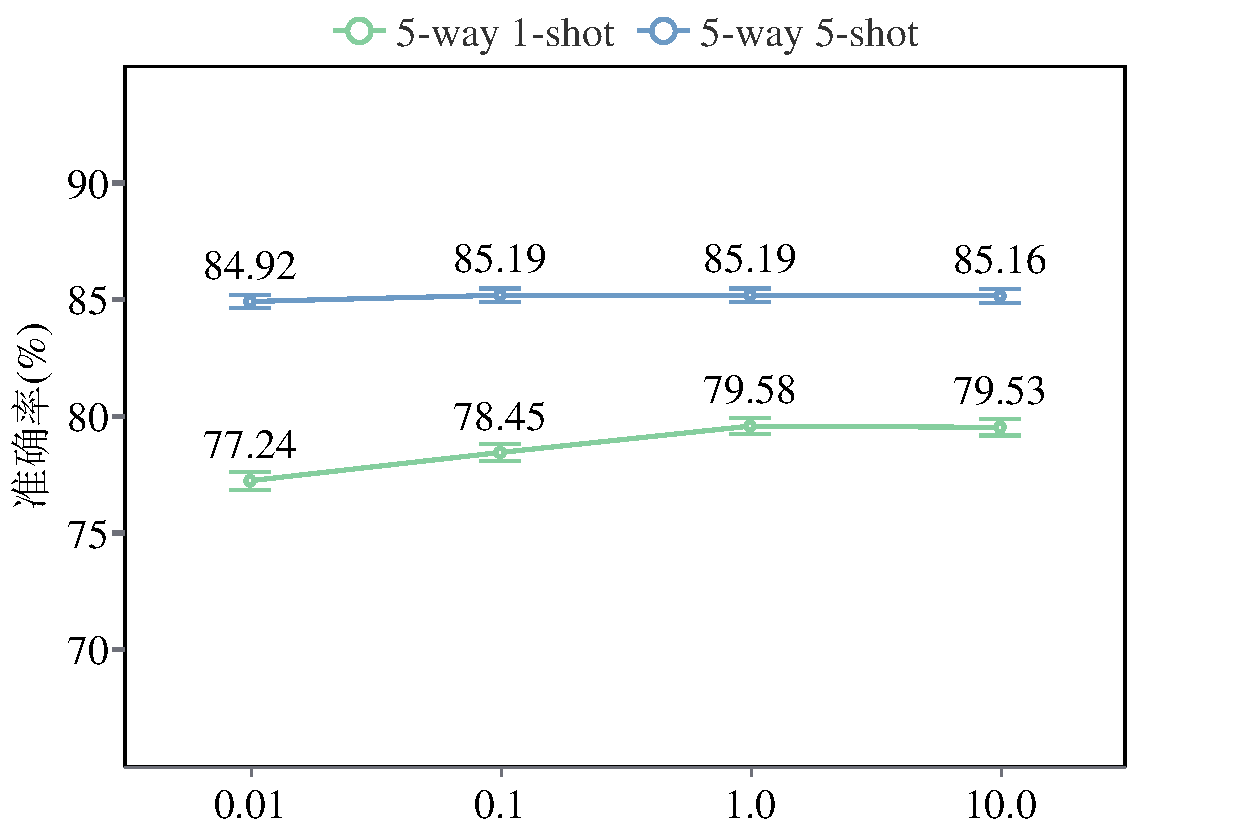
\includegraphics[width=0.6\columnwidth]{figures/SVMSMA/miniImageNet/alpha.pdf}
  \bicaption[SVMSMA在miniImageNet数据集上的超参数$\alpha$消融实验]{SVMSMA在miniImageNet数据集上的超参数$\alpha$消融实验。}[Hyperparameter $\alpha$ ablation experiments of SVMSMA on miniImageNet]{Hyperparameter $\alpha$ ablation experiments of SVMSMA on miniImageNet.}
  \label{figure4: alpha (miniImageNet)}
  % \vspace{-4pt}
\end{figure}

\begin{figure}[h!]
  \centering
  \captionsetup{font={small, stretch=1.312}}
  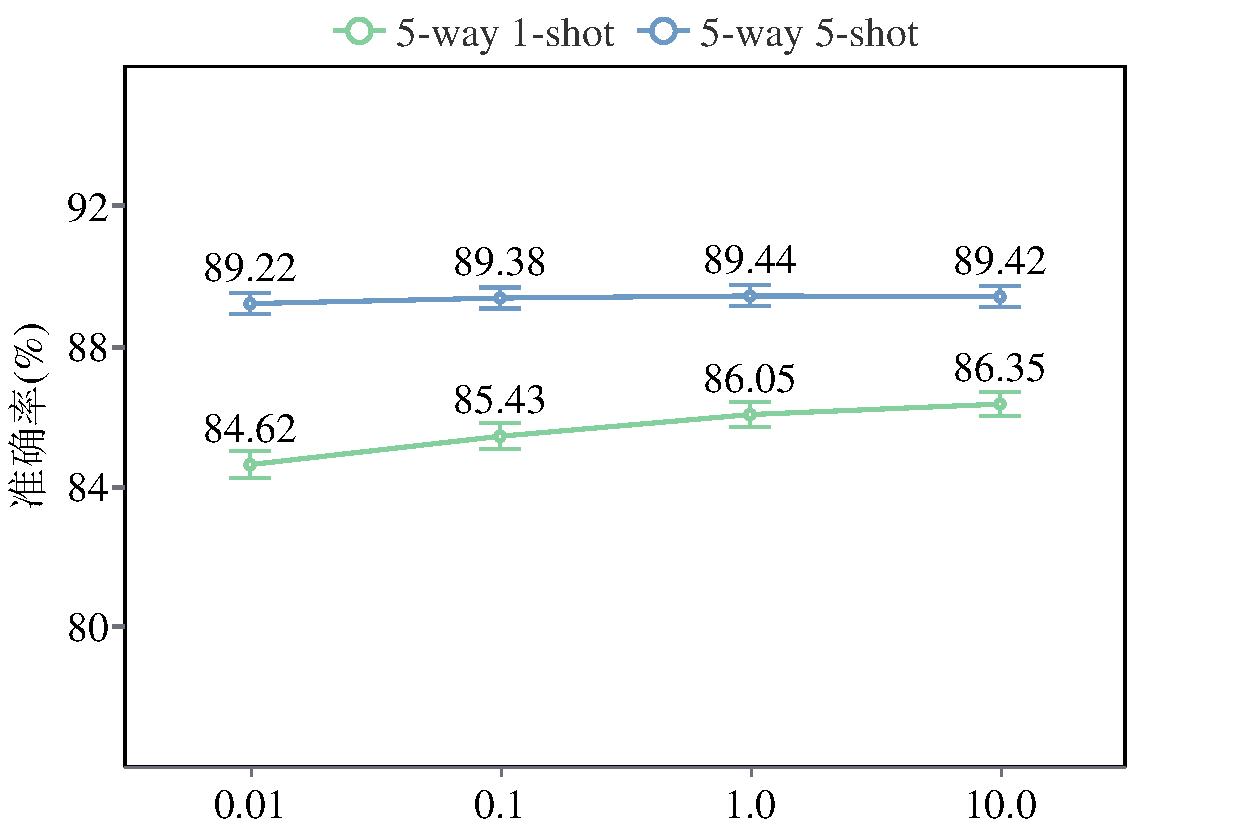
\includegraphics[width=0.6\columnwidth]{figures/SVMSMA/CIFAR-FS/alpha.pdf}
  \bicaption[SVMSMA在CIFAR-FS数据集上的超参数$\alpha$消融实验]{SVMSMA在CIFAR-FS数据集上的超参数$\alpha$消融实验。}[Hyperparameter $\alpha$ ablation experiments of SVMSMA on CIFAR-FS]{Hyperparameter $\alpha$ ablation experiments of SVMSMA on CIFAR-FS.}
  \label{figure4: alpha (CIFAR-FS)}
  % \vspace{-4pt}
\end{figure}

\begin{figure}[h!]
  \centering
  \captionsetup{font={small, stretch=1.312}}
  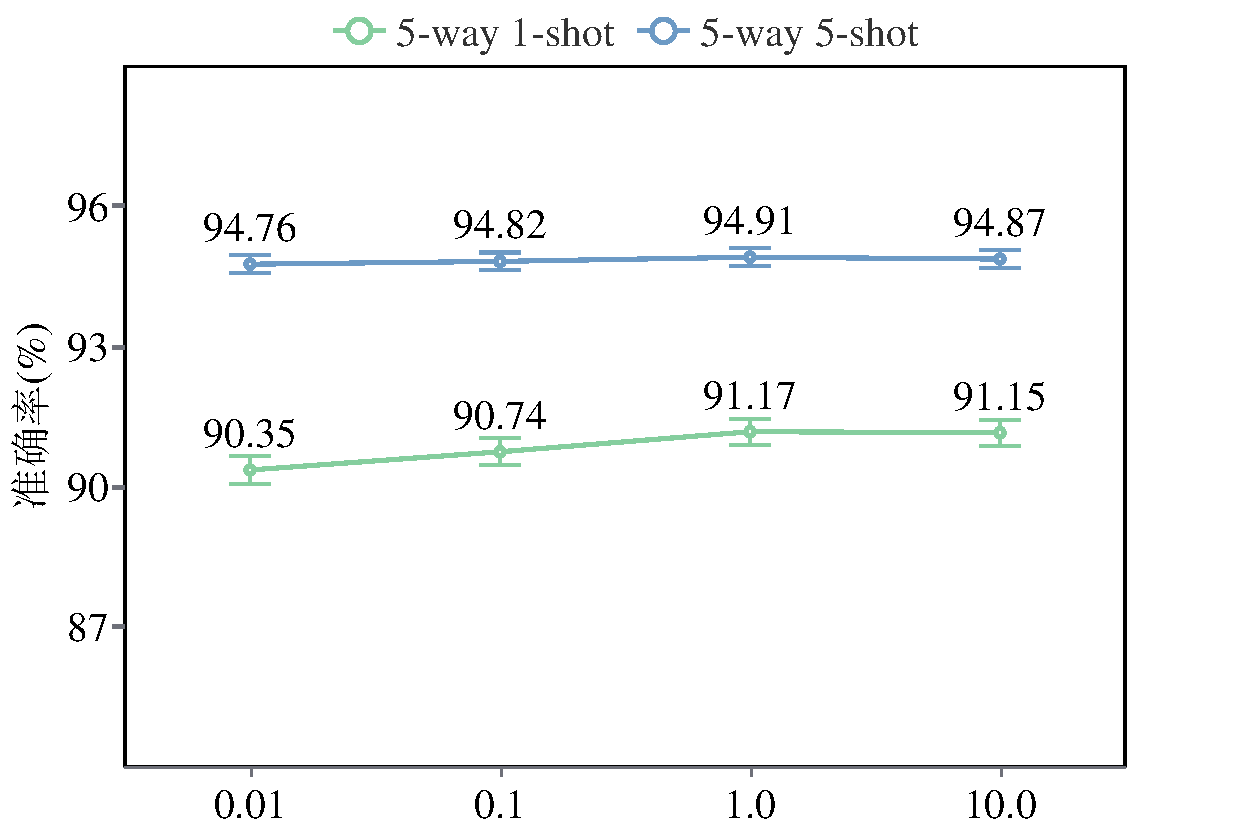
\includegraphics[width=0.6\columnwidth]{figures/SVMSMA/CUB/alpha.pdf}
  \bicaption[SVMSMA在CUB数据集上的超参数$\alpha$消融实验]{SVMSMA在CUB数据集上的超参数$\alpha$消融实验。}[Hyperparameter $\alpha$ ablation experiments of SVMSMA on CUB]{Hyperparameter $\alpha$ ablation experiments of SVMSMA on CUB.}
  \label{figure4: alpha (CUB)}
  % \vspace{-4pt}
\end{figure}

\textbf{(2)讨论超参数对模型性能的影响}

$\alpha$是调整不同损失权重占比的超参数,本文通过将其设置为不同数值来讨论$\alpha$对模型的影响,同样在miniImageNet、CIFAR-FS、CUB三个数据集进行了实验分析。

如图\ref{figure4: alpha (miniImageNet)}、\ref{figure4: alpha (CIFAR-FS)}和\ref{figure4: alpha (CUB)}所示,对于miniImageNet和CUB数据集,无论是5-way 1-shot还是5-way 5-shot任务,模型均在将$\alpha$设置为1.0时达到最优结果,因此对于这两个数据集,$\alpha$被设置为1.0。而对于CIFAR-FS数据集,5-way 1-shot任务在$\alpha = 10.0$时取得最优结果,5-way 5-shot任务则是在$\alpha = 1.0$取得最优结果,但5-shot任务准确率差别很微小,因此在CIFAR-FS数据集上,超参数$\alpha$被设置为10.0。此外,超参数$\alpha$被设置为0.1、1.0与10.0时,模型结果变化较小,这证明了所提方法对超参数$\alpha$的稳定性。

\begin{table}[h!]
  \small    % 设置表格字体为5号
  \setstretch{1.245}        % 设置具有指定弹力的橡皮长度(原行宽的1.2倍)
  \captionsetup{font={small, stretch=1.512}}
  \centering
  % \vspace{-10pt}
  \bicaption[SVMSMA在miniImageNet、CIFAR-FS和CUB数据集上的不同特征消融实验]{SVMSMA在miniImageNet、CIFAR-FS和CUB数据集上的不同特征消融实验。最优结果用粗体表示。}{Different features ablation experiments of SVMSMA on miniImageNet, CIFAR-FS and CUB. The best results are shown in bold.}    % 中英文标题
  \begin{tabularx}{\textwidth}{ClCC}
    \toprule
    数据集 & 特征      & 5-way 1-shot              & 5-way 5-shot              \\
    \midrule
    \multirow{4}{*}{miniImageNet}
        & 视觉特征    & 69.57 $\pm$ 0.45          & 84.41 $\pm$ 0.30          \\
        & 单模态映射特征 & 73.73 $\pm$ 0.39          & 73.83 $\pm$ 0.39          \\
        & 多模态映射特征 & 78.34 $\pm$ 0.37          & 81.29 $\pm$ 0.34          \\
        & SVMSMA  & \textbf{79.58 $\pm$ 0.35} & \textbf{85.19 $\pm$ 0.29} \\
    \midrule
    \multirow{4}{*}{CIFAR-FS}
        & 视觉特征    & 78.54 $\pm$ 0.47          & 88.64 $\pm$ 0.32          \\
        & 单模态映射特征 & 83.44 $\pm$ 0.37          & 83.60 $\pm$ 0.38          \\
        & 多模态映射特征 & 86.00 $\pm$ 0.36          & 87.40 $\pm$ 0.33          \\
        & SVMSMA  & \textbf{86.35 $\pm$ 0.35} & \textbf{89.42 $\pm$ 0.30} \\
    \midrule
    \multirow{4}{*}{CUB}
        & 视觉特征    & 86.14 $\pm$ 0.38          & 94.75 $\pm$ 0.19          \\
        & 单模态映射特征 & 83.58 $\pm$ 0.43          & 83.53 $\pm$ 0.43          \\
        & 多模态映射特征 & 89.90 $\pm$ 0.31          & 93.60 $\pm$ 0.22          \\
        & SVMSMA  & \textbf{91.17 $\pm$ 0.28} & \textbf{94.91 $\pm$ 0.19} \\
    \bottomrule
  \end{tabularx}
  % \vspace{-25pt}
  \label{table4: modal ablation}
\end{table}

\textbf{(3)讨论不同映射模式特征的分类准确率}

如\ref{section4: 语义-视觉多空间映射网络}所述,根据映射网络输入特征模态不同,可将其分为两种模式:单模态映射和多模态映射。为讨论不同映射模式特征对少样本分类结果的影响,本文进行了实验分析。

如表\ref{table4: modal ablation}所示,对于5-way 1-shot任务,无论是单模态映射特征,还是多模态映射特征,均取得了较视觉特征高的准确率。这证明了利用语义特征可以更好地建立新类与基类之间联系,从而迁移在基类上学习到的知识,也证明了语义信息对少样本分类的重要性。另外,在将三个特征共同作为分类器的训练数据时,模型能够取得进一步的效果提升。对于5-way 5-shot任务,相对于视觉特征,单模态映射特征和多模态映射特征的准确率均有所降低,尤其是单模态映射特征,降低幅度尤为明显。导致这种现象出现的原因是因为每个类别的语义特征以及视觉原型特征都是固定的,将其映射到视觉空间并执行分类与特征对齐任务会使其得模型学习到一个投影相对固定的映射网络,即映射后特征的多样性会较差。因此即使其更接近类别中心,但由于多样性差会导致其不如使用多样性较好的视觉特征训练出来的分类边界更加鲁棒,导致取得较差的5-shot任务结果。虽然多模态映射模式中将视觉特征与语义特征共同输入网络缓解了这种情况,但仍比视觉特征的分类准确率低。本文通过使用三种特征一起训练分类器,利用视觉特征的多样性解决了此问题,取得了较使用单一特征更好的结果。


\begin{table}[h!]
  \small    % 设置表格字体为5号
  \setstretch{1.245}        % 设置具有指定弹力的橡皮长度(原行宽的1.2倍)
  \captionsetup{font={small, stretch=1.512}}
  \centering
  % \vspace{-10pt}
  \bicaption[SVMSMA在miniImageNet、CIFAR-FS和CUB数据集上的不同语义特征消融实验]{SVMSMA在miniImageNet、CIFAR-FS和CUB数据集上的不同语义特征消融实验。最优结果用粗体表示。}{Different semantic features ablation experiments of SVMSMA on miniImageNet, CIFAR-FS and CUB. The best results are shown in bold.}    % 中英文标题
  \begin{tabularx}{\textwidth}{ClCC}
    \toprule
    数据集 & 方法                  & 5-way 1-shot              & 5-way 5-shot              \\
    \midrule
    \multirow{4}{*}{miniImageNet}
        & Baseline            & 69.57 $\pm$ 0.45          & 84.41 $\pm$ 0.30          \\
        & SVMSMA-GloVe (name) & 71.53 $\pm$ 0.46          & 81.49 $\pm$ 0.34          \\
        & SVMSMA-SBERT (name) & 73.29 $\pm$ 0.43          & 82.94 $\pm$ 0.32          \\
        & SVMSMA-CLIP (name)  & 78.16 $\pm$ 0.37          & 84.93 $\pm$ 0.28          \\
        & SVMSMA-CLIP (text)  & \textbf{79.58 $\pm$ 0.35} & \textbf{85.19 $\pm$ 0.29} \\
    \midrule
    \multirow{4}{*}{CIFAR-FS}
        & Baseline            & 78.54 $\pm$ 0.47          & 88.64 $\pm$ 0.32          \\
        & SVMSMA-GloVe (name) & 83.19 $\pm$ 0.40          & 88.25 $\pm$ 0.32          \\
        & SVMSMA-SBERT (name) & 82.24 $\pm$ 0.41          & 88.15 $\pm$ 0.31          \\
        & SVMSMA-CLIP (name)  & 85.34 $\pm$ 0.37          & 89.24 $\pm$ 0.30          \\
        & SVMSMA-CLIP (text)  & \textbf{86.35 $\pm$ 0.35} & \textbf{89.42 $\pm$ 0.30} \\
    \midrule
    \multirow{4}{*}{CUB}
        & Baseline            & 86.14 $\pm$ 0.38          & 94.75 $\pm$ 0.19          \\
        & SVMSMA-GloVe (name) & 87.67 $\pm$ 0.35          & 93.83 $\pm$ 0.21          \\
        & SVMSMA-SBERT (name) & 87.40 $\pm$ 0.35          & 94.20 $\pm$ 0.20          \\
        & SVMSMA-CLIP (name)  & 91.06 $\pm$ 0.28          & \textbf{94.91 $\pm$ 0.19} \\
        & SVMSMA-CLIP (text)  & \textbf{91.17 $\pm$ 0.28} & \textbf{94.91 $\pm$ 0.19} \\
    \bottomrule
  \end{tabularx}
  \label{table4: text encoder ablation}
\end{table}

\textbf{(4)讨论不同语义特征提取网络对模型性能的影响}

为了进一步证明本文方法的可推广性,本文也使用其他模型作为语义特征提取网络:GloVe与SBERT,对于这两个模型,本文使用类别名称作为模型的输入,因此表示为SVMSMA-GloVe (name)与SVMSMA-SBERT (name)。

如表\ref{table4: text encoder ablation}所示,在1-shot任务上,SVMSMA-GloVe与SVMSMA-SBERT都通过提高样本特征多样性的手段取得了优于基准模型的表现,从而进一步证明了语义特征对于少样本分类问题的重要性以及本文方法的可迁移性。而在5-shot任务上,模型性能均有所降低,尤其是在miniImageNet数据集上。这是因为这两个模型提取的语义特征迁移性不够好,语义映射特征并不像使用CLIP模型时具有代表性,原本较多数量的视觉特征便可以使分类器学习到良好分类边界,而增加了这些样本会对样本特征空间造成一定的干扰,使其偏离原本分类边界,且为向远离真实分类边界的方向偏离,造成性能下降。虽说通过调整各种特征的比例能够缓解或避免这种现象,但为了方法的简易性,对此部分内容本文不再进行描述。

此外,本文也讨论了是否使用提示文本对模型性能的影响,使用类别名称作为CLIP文本编码器输入进行了实验。使用类别名称作为输入时,模型表示为SVMSMA-CLIP (name),添加提示文本时则表示为SVMSMA-CLIP (text),如表\ref{table4: text encoder ablation}所示。可以观察到,虽然SVMSMA-CLIP (name)模型也取得了优异的效果,但仍不如添加提示文本后模型表现,在miniImageNet、CIFAR-FS和CUB三个数据集1-shot任务上分别降低了1.42\%、1.01\%和0.11\%的准确率,在5-shot任务也有略微降低。这一实验证明了提示文本对模型表现具有一定影响,也为将来通过设计提示文本或将其参数化进一步提升模型性能提供了依据。

\begin{figure}[h!]
  \centering
  \captionsetup{font={small, stretch=1.312}}
  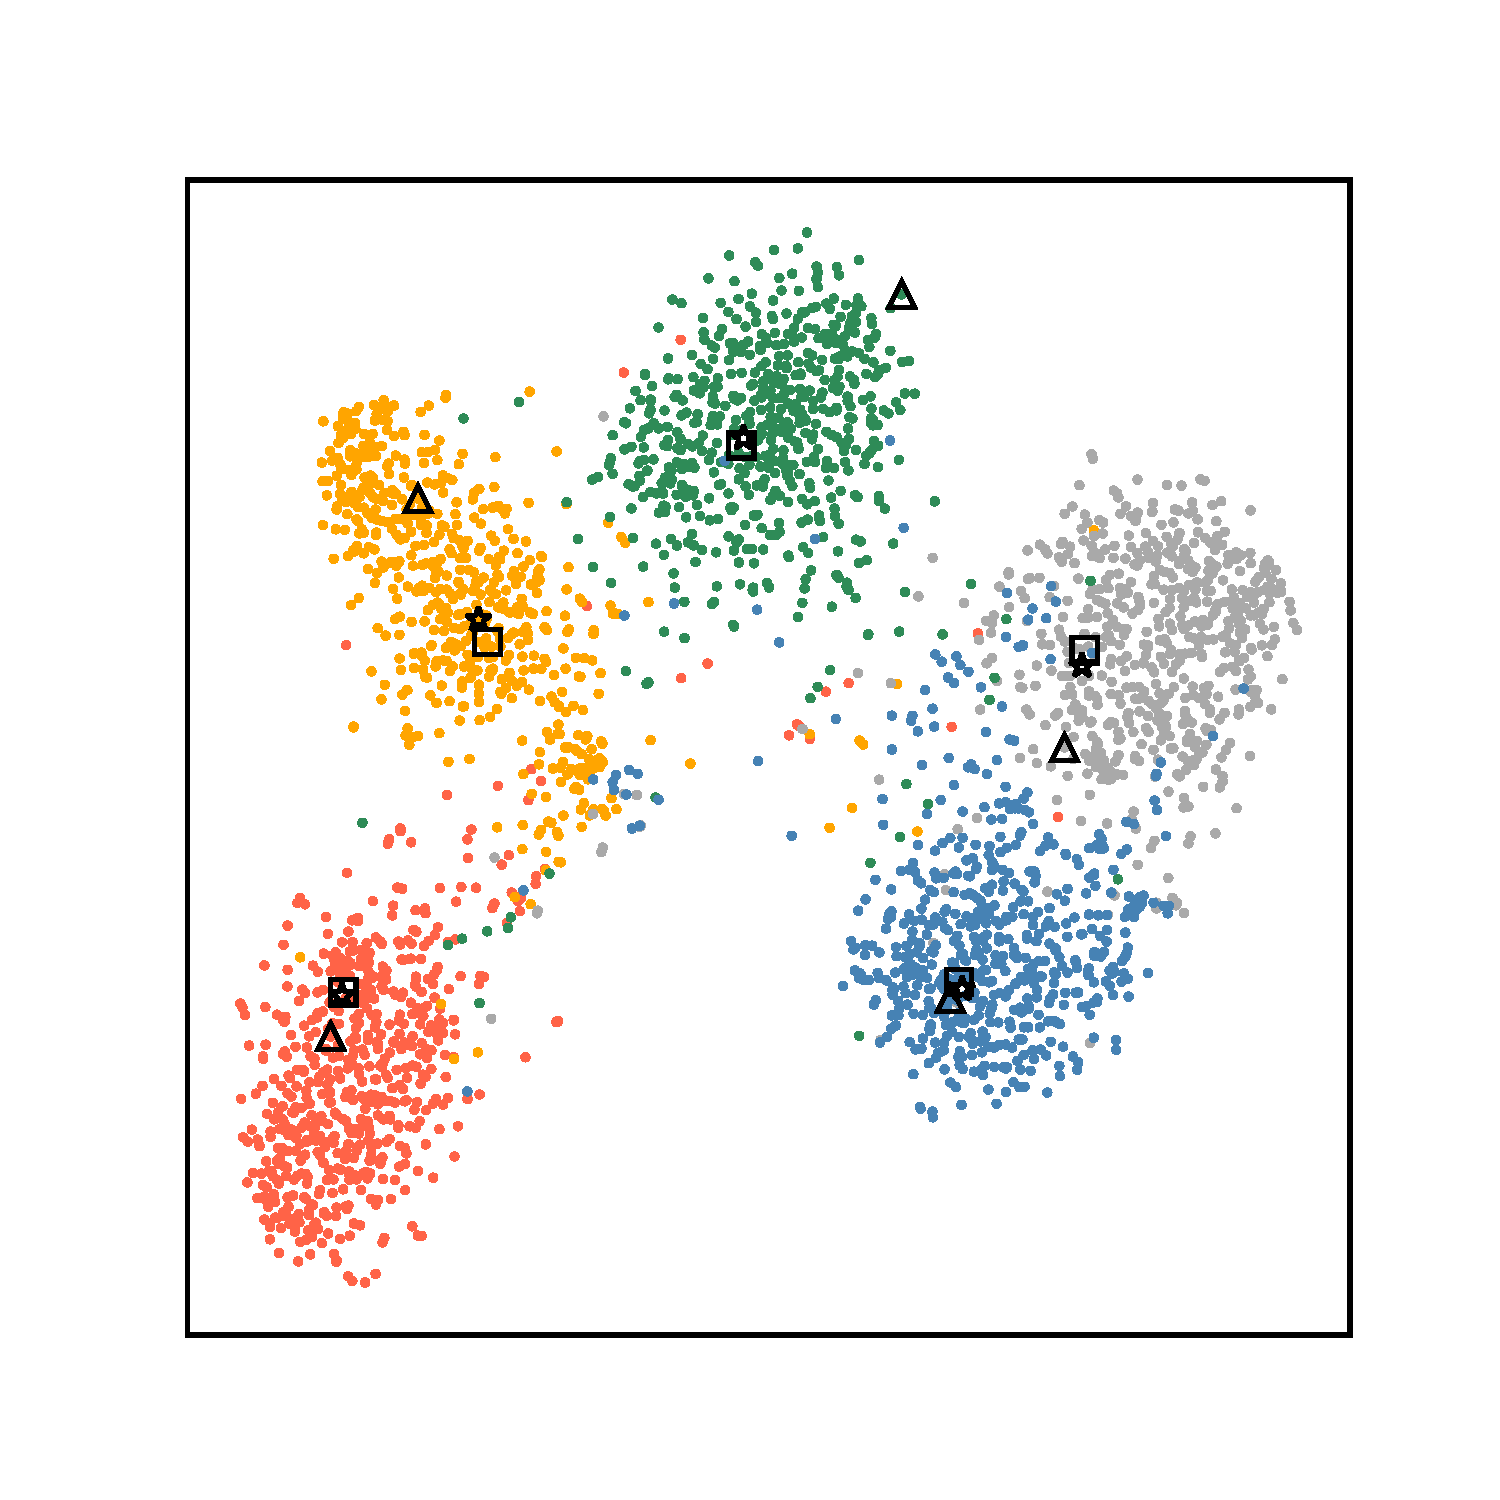
\includegraphics[width=0.5\columnwidth]{figures/SVMSMA/miniImageNet/t-SNE.pdf}
  \bicaption[miniImageNet数据集上不同特征的t-SNE可视化结果]{miniImageNet数据集上不同特征的t-SNE可视化结果。不同颜色代表不同类别。视觉特征、单模态映射特征、多模态映射特征分别用$\triangle$、$\Box$和$\hollowstar$表示。}[The t-SNE visualization results of different features on miniImageNet]{The t-SNE visualization results of different features on miniImageNet. Different colors represent different categories. visual features, single-modal mapping features, and multi-modal mapping features are represented by $\triangle$, $\Box$, and $\hollowstar$, respectively.}
  \label{figure4: t-SNE}
\end{figure}

\subsection[\hspace{-2pt}可视化分析]{{\heiti\zihao{4} \hspace{-8pt}可视化分析}}\label{section4: 可视化分析}

为了更好地展示SVMSMA方法能够通过引入语义特征对视觉特征进行补充,本文在miniImageNet数据集上随机选取了5个新类并使用t-SNE对每个类别所有样本的视觉特征,随机选取一个5-way 1-shot任务支持集样本的视觉特征($\triangle$)、单模态映射特征($\Box$)、多模态映射特征($\hollowstar$)进行了可视化实验,如图\ref{figure4: t-SNE}所示。在此图里,可以看到无论是单模态特征还是多模态特征都能较好地落在样本簇中,这使得将它们加入逻辑回归器的训练数据可以提升支持集样本特征的多样性,从而在查询集上达到更好的分类效果。另外,在某些较为极端的情况下,如图中绿色类别和灰色类别所示,支持集样本视觉特征处于类别边缘或者分类边界。对于这种情况,如果单独使用视觉特征一般会取得较差的分类结果。而使用本文提出方法所获取的单模态映射特征和多模态映射特征则处于样本簇较为中央的位置,从而能够校正视觉特征造成的偏差,优化分类器学习到的分类边界,达到更好的准确率。综上所述,SVMSMA方法能够使用语义信息对视觉信息进行补充,通过增加支持集样本的方式丰富支持集样本的多样性,同时对视觉特征处于样本簇边缘时造成的分类边界偏差进行修正,从而提高少样本分类任务的准确率。


\section[\hspace{-2pt}本章小结]{{\heiti\zihao{-3} \hspace{-8pt}本章小结}}\label{section4: 本章小结}

本章研究基于语义-视觉多空间关系建模的少样本特征适配算法,针对少样本分类中仅根据少量视觉特征无法捕获类别代表性特征的缺点,引入语义信息作为视觉信息的补充,通过对语义-视觉多空间关系进行建模,提出了语义-视觉多空间映射适配模型(Semantic-Visual Multi-Space Mapping Adapter,简称SVMSMA),以丰富样本特征的信息来源,利用语义特征对视觉特征进行补充与修正,从而提升模型在新类上的泛化能力。SVMSMA模型使用单/多模态映射网络将样本语义特征映射到视觉空间获得单/多模态映射特征,并通过跨模态分类(CMC)模块与跨模态特征对齐(CMFA)模块对映射网络进行优化,以使得语义特征与视觉特征建立联系。测试过程中,本章方法将支持集的视觉特征、单模态映射特征、以及多模态映射特征共同作为分类器的训练数据,达到了较仅使用单一特征时更好的分类结果。在miniImageNet、tieredImageNet、CIFAR-FS和CUB-200-2011数据集的大量实验表明了SVMSMA方法的有效性。

综上所述,本章提出的基于语义-视觉多空间关系建模的少样本特征适配算法通过对语义-视觉多空间关系进行建模,充分利用语义信息对视觉信息进行了补充,丰富了样本特征信息来源,提升了模型的泛化能力。
